\documentclass[a4paper, 12pt]{article}
% (Includi qui i pacchetti e le impostazioni necessarie...)

\newcommand{\template}{../../Templates}
\usepackage{\template/package}
\graphicspath{{../../Assets}}

\newcommand{\Titolo}{Norme di progetto}
\newcommand{\Data}{21/11/2023}
\newcommand{\Versione}{1.3.0}
\newcommand{\Descrizione}{Elenco delle procedure interne e delle buone pratiche 
di progetto adottate dal gruppo.}
\newcommand{\Verificatori}{Niccolò Carlesso}
\newcommand{\Stato}{Non approvato}

\newcommand{\Gruppo}{SWEnergy}
\newcommand{\Mail}{\href{mailto:project.swenergy@gmail.com}{project.swenergy@gmail.com}}

\renewcommand\familydefault{\sfdefault} % Set default font family to sans-serif
\linespread{1.5}

\hypersetup{
	pdfmenubar=true,            % show Acrobat’s menu?
	pdfstartview={FitH},        % fits the width of the page to the window
	colorlinks=true,            % false: boxed links; true: colored links
	linkcolor=black,            % color of internal links (change box color with linkbordercolor)
	% citecolor=green,          % color of links to bibliography
	% filecolor=magenta,        % color of file links
	urlcolor=[RGB]{156,1,198}   % color of external links
}

\newcommand{\copertina}{
	\begin{titlepage}
		\vspace*{-3.5cm}
		\makebox[\textwidth]{
\includegraphics[width=\paperwidth]{header.png}}
		\begin{center}
			
\includegraphics[width=1\textwidth]{logo.png}	\\
			\vspace{1cm}
			\Mail	\\
			\vspace{0.5cm}
			\textbf{\begin{LARGE} \Titolo \end{LARGE}}		\\
			\vspace{1cm}
			\textbf{Descrizione:} \Descrizione{}			\\
			\vspace{1cm}
			\begin{tabular}{ll}
				\textbf{Stato}               & \Stato              \\
				\textbf{Data}                & \Data               \\
				\midrule
				\textbf{Redattori}           & \Redattori          \\
				\textbf{Verificatori}        & \Verificatori       \\

				\ifdefined\Approvatori
				\textbf{Approvatori}         & \Approvatori        \\
				\fi

				\ifdefined\ApprovatoriInterni
				\textbf{Approvatori interni} & \ApprovatoriInterni \\
				\fi

				\ifdefined\ApprovatoriEsterni
				\textbf{Approvatori esterni} & \ApprovatoriEsterni \\
				\fi

				\ifdefined\Destinatari
				\textbf{Destinatari}         & \Destinatari        \\
				\fi

				\midrule

				\ifdefined\Versione
				\textbf{Versione}            & \Versione           \\
				\fi
			\end{tabular}
		\end{center}
		\vspace{4cm}
	\end{titlepage}
	\newpage
}

\fancypagestyle{plain}{
	\fancyhf{}
	\rhead{ 
\includegraphics[scale=0.05]{horizontal_logo.png}}
	\lhead{\Titolo \ifdefined\Versione \ \Versione \fi}
	%\lfoot{\Titolo}
	\rfoot{\thepage{} di \pageref{LastPage}}
	\renewcommand{\headrulewidth}{0.2pt}
	\renewcommand{\footrulewidth}{0.2pt}
}
\pagestyle{plain}


\begin{document}
\copertina{}
\section*{Registro delle modifiche}
 {
  \scriptsize
  \begin{tabular}{p{0.10\linewidth}p{0.10\linewidth}p{0.15\linewidth}p{0.15\linewidth}p{0.15\linewidth}p{0.19\linewidth}}
	  \textbf{Versione} & \textbf{Data} & \textbf{Redattore}     & \textbf{Verificatore} & \textbf{Approvatore} & \textbf{Descrizione}                                                                                                                     \\
	  \toprule
	  2.0.1             & 27/02/2024    & Davide Maffei          & Carlo Rosso           & /                    & Correzioni in seguito alla revisione RTB                                                                                                 \\
	  \hline
	  2.0.0             & 27/02/2024    & /                      & /                     & Niccolò Carlesso     & Approvazione finale del documento                                                                                                        \\
	  \hline
	  1.5.0             & 26/02/2024    & Alessandro Tigani Sava & Carlo Rosso           & /                    & Descrizione metriche di qualità                                                                                                          \\
	  \hline
	  1.4.1             & 14/02/2024    & Davide Maffei          & Giacomo Gualato       & /                    & Allineamento delle sezioni dei ruoli                                                                                                     \\
	  \hline
	  1.4.0             & 14/02/2024    & Davide Maffei          & Giacomo Gualato       & /                    & Creazione delle sezioni dei processi primari, di supporto e organizzativi                                                                \\
	  \hline
	  1.3.0             & 8/01/2024     & Carlo Rosso            & Niccolò Carlesso      & /                    & Correzione della sotto-sezione "Aggiornamento delle "Norme di Progetto"" e aggiunte le sotto-sezioni "Revisione del codice" e "Codifica" \\
	  \hline
	  1.2.0             & 31/12/2023    & Carlo Rosso            & Niccolò Carlesso      & /                    & Ristrutturazione del documento per ruolo, piuttosto che per argomento                                                                    \\
	  \hline
	  1.1.0             & 30/10/2023    & Carlo Rosso            & Giacomo Gualato       & /                    & Aggiornamento della sezione dedicata alla documentazione e aggiunta una sezione dedicata agli appunti                                    \\
	  \hline
	  1.0.0             & 30/10/2023    & /                      & /                     & Giacomo Gualato      & Approvazione finale del documento                                                                                                        \\
	  \hline
	  0.2.1             & 29/10/2023    & Alessandro Tigani Sava & Niccolò Carlesso      & /                    & Modifica procedure in sezione Approvazione di un documento                                                                               \\
	  \hline
	  0.2.0             & 24/10/2023    & Matteo Bando           & Niccolò Carlesso      & /                    & Redazione sezioni Versionamento, Verifica di un documento, Approvazione di un documento                                                  \\
	  \hline
	  0.1.0             & 23/10/2023    & Alessandro Tigani Sava & Matteo Bando          & /                    & Redazione sezioni Introduzione, Strumenti, Creazione e modifica di un documento, Ruoli, Registro delle modifiche                         \\
	  \hline
  \end{tabular}
 }

\newpage

\setcounter{tocdepth}{2}
\tableofcontents
\newpage
\section{Introduzione}

Il presente documento, intitolato "Piano di Progetto", descrive e spiegare le
decisioni organizzative adottate dal gruppo SWEnergy per lo sviluppo del
progetto "\textit{Easy Meal}", proposto dall'azienda
\href{https://imolainformatica.it/}{Imola Informatica}. Il "Piano di Progetto" è
suddiviso nelle seguenti sezioni:

\begin{itemize}
	\item \textbf{Analisi dei rischi}: identifica i rischi individuati dal
	      gruppo e le strategie per mitigarli;

	\item \textbf{Modello di sviluppo}: descrive l'organizzazione temporale del
	      team di SWEnergy;

	\item \textbf{Pianificazione}: dettaglia la pianificazione del lavoro del
	      gruppo, incluse le attività, le risorse e i tempi necessari per lo
	      sviluppo del progetto;

	\item \textbf{Preventivo}: presenta il preventivo delle ore di lavoro e il
	      costo totale del progetto;

	\item \textbf{Consuntivo}: riporta le ore di lavoro e il costo effettivo del
	      progetto fino al momento della stesura del piano di progetto della
	      fase corrente: RTB.
\end{itemize}

\subsection{Scopo del documento}

Questo documento ha lo scopo di raccogliere in modo organico, coerente e
uniforme tutte le informazioni riguardanti la pianificazione del progetto, al
fine di fornire un riferimento per la gestione dello stesso. Al termine della
prima fase del progetto (RTB), verrà utilizzato per valutare l'andamento del
lavoro e per spiegare le decisioni adottate durante la pianificazione.

\subsection{Scopo del prodotto}

"\textit{Easy Meal}" è una web app progettata per gestire le prenotazioni
presso i ristoranti, sia dal lato dei clienti che dei ristoratori. Il prodotto
finale sarà composto da due parti:

\begin{itemize}
	\item \textbf{Cliente}: consente ai clienti di prenotare un tavolo presso un
	      ristorante, visualizzare il menù e effettuare un ordine;

	\item \textbf{Ristoratore}: consente ai ristoratori di gestire le
	      prenotazioni e gli ordini dei clienti, oltre a visualizzare la lista
	      degli ingredienti necessari per preparare i piatti ordinati.
\end{itemize}

\subsection{Glossario}

Al fine di evitare ambiguità linguistiche e garantire un'utilizzazione coerente
delle terminologie nei documenti, il gruppo ha redatto un documento interno
chiamato "Glossario". Questo documento definisce in modo chiaro e preciso i
termini che potrebbero generare ambiguità o incomprensione nel testo. I termini
presenti nel Glossario sono identificati da una 'G' (per esempio parola$_G$) a
pedice.

\subsection{Riferimenti}

\subsubsection{Normativi}
\begin{itemize}
	\item "\textit{Way of Working}";
	\item 	\href{https://www.math.unipd.it/~tullio/IS-1/2023/Progetto/C3.pdf}
	      {Documento del capitolato d'appalto C3 - \textit{Easy Meal}};
	\item \href{https://www.math.unipd.it/~tullio/IS-1/2023/Dispense/PD2.pdf}
	      {Regolamento del progetto};
\end{itemize}

\subsubsection{Informativi}

Slide dell'insegnamento di Ingegneria del Software:
\begin{itemize}
	\item \href{https://www.math.unipd.it/~tullio/IS-1/2023/Dispense/T3.pdf}
	      {Modelli di sviluppo del software};
	\item \href{https://www.math.unipd.it/~tullio/IS-1/2023/Dispense/T4.pdf}
	      {Gestione di progetto};
	\item \href{https://www.math.unipd.it/~tullio/IS-1/2023/Dispense/T5.pdf}
	      {Analisi dei requisiti};
\end{itemize}

\subsection{Scadenze}
Il \textit{team} di SWEnergy si impegna a rispettare le seguenti scadenze per il
completamento del progetto:
\begin{itemize}
	\item \textbf{Prima revisione (avanzamento RTB}: 21 dicembre 2023;
	\item \textbf{Seconda revisione (avanzamento PB)}: da definire;
	\item \textbf{Terza revisione (avanzamento CA)}: da definire;
\end{itemize}

\newpage

\section{Introduzione}

Il presente documento, intitolato "Piano di Progetto", descrive e spiegare le
decisioni organizzative adottate dal gruppo SWEnergy per lo sviluppo del
progetto "\textit{Easy Meal}", proposto dall'azienda
\href{https://imolainformatica.it/}{Imola Informatica}. Il "Piano di Progetto" è
suddiviso nelle seguenti sezioni:

\begin{itemize}
	\item \textbf{Analisi dei rischi}: identifica i rischi individuati dal
	      gruppo e le strategie per mitigarli;

	\item \textbf{Modello di sviluppo}: descrive l'organizzazione temporale del
	      team di SWEnergy;

	\item \textbf{Pianificazione}: dettaglia la pianificazione del lavoro del
	      gruppo, incluse le attività, le risorse e i tempi necessari per lo
	      sviluppo del progetto;

	\item \textbf{Preventivo}: presenta il preventivo delle ore di lavoro e il
	      costo totale del progetto;

	\item \textbf{Consuntivo}: riporta le ore di lavoro e il costo effettivo del
	      progetto fino al momento della stesura del piano di progetto della
	      fase corrente: RTB.
\end{itemize}

\subsection{Scopo del documento}

Questo documento ha lo scopo di raccogliere in modo organico, coerente e
uniforme tutte le informazioni riguardanti la pianificazione del progetto, al
fine di fornire un riferimento per la gestione dello stesso. Al termine della
prima fase del progetto (RTB), verrà utilizzato per valutare l'andamento del
lavoro e per spiegare le decisioni adottate durante la pianificazione.

\subsection{Scopo del prodotto}

"\textit{Easy Meal}" è una web app progettata per gestire le prenotazioni
presso i ristoranti, sia dal lato dei clienti che dei ristoratori. Il prodotto
finale sarà composto da due parti:

\begin{itemize}
	\item \textbf{Cliente}: consente ai clienti di prenotare un tavolo presso un
	      ristorante, visualizzare il menù e effettuare un ordine;

	\item \textbf{Ristoratore}: consente ai ristoratori di gestire le
	      prenotazioni e gli ordini dei clienti, oltre a visualizzare la lista
	      degli ingredienti necessari per preparare i piatti ordinati.
\end{itemize}

\subsection{Glossario}

Al fine di evitare ambiguità linguistiche e garantire un'utilizzazione coerente
delle terminologie nei documenti, il gruppo ha redatto un documento interno
chiamato "Glossario". Questo documento definisce in modo chiaro e preciso i
termini che potrebbero generare ambiguità o incomprensione nel testo. I termini
presenti nel Glossario sono identificati da una 'G' (per esempio parola$_G$) a
pedice.

\subsection{Riferimenti}

\subsubsection{Normativi}
\begin{itemize}
	\item "\textit{Way of Working}";
	\item 	\href{https://www.math.unipd.it/~tullio/IS-1/2023/Progetto/C3.pdf}
	      {Documento del capitolato d'appalto C3 - \textit{Easy Meal}};
	\item \href{https://www.math.unipd.it/~tullio/IS-1/2023/Dispense/PD2.pdf}
	      {Regolamento del progetto};
\end{itemize}

\subsubsection{Informativi}

Slide dell'insegnamento di Ingegneria del Software:
\begin{itemize}
	\item \href{https://www.math.unipd.it/~tullio/IS-1/2023/Dispense/T3.pdf}
	      {Modelli di sviluppo del software};
	\item \href{https://www.math.unipd.it/~tullio/IS-1/2023/Dispense/T4.pdf}
	      {Gestione di progetto};
	\item \href{https://www.math.unipd.it/~tullio/IS-1/2023/Dispense/T5.pdf}
	      {Analisi dei requisiti};
\end{itemize}

\subsection{Scadenze}
Il \textit{team} di SWEnergy si impegna a rispettare le seguenti scadenze per il
completamento del progetto:
\begin{itemize}
	\item \textbf{Prima revisione (avanzamento RTB}: 21 dicembre 2023;
	\item \textbf{Seconda revisione (avanzamento PB)}: da definire;
	\item \textbf{Terza revisione (avanzamento CA)}: da definire;
\end{itemize}


\section{Processi Primari}

Qui bisogna scrivere che cosa sono i processi primari.

\subsection{Acquisizione}

Il processo di acquisizione coinvolge la definizione dei requisiti di sistema e
\textit{software}, la valutazione e selezione dei potenziali fornitori, e la gestione del
contratto con il fornitore selezionato.

\subsubsection{Scopo}
Garantire che il \textit{software} acquisito soddisfi i requisiti stabiliti, rispetti i
vincoli di budget e di tempo, e sia conforme agli \textit{standard} di qualità previsti.

\subsubsection{Attività}
\subsubsubsection{Definizione dei requisiti} 
Identificazione delle necessità e delle aspettative degli \textit{stakeholder};

\subsubsubsection{Selezione del fornitore} 
Valutazione delle offerte e scelta del fornitore più adatto;

\subsubsubsection{Gestione del contratto} 
Definizione degli accordi contrattuali, monitoraggio della conformità e gestione 
delle modifiche;

\subsubsubsection{Accettazione del \textit{software}} 
Verifica e approvazione del \textit{software} consegnato rispetto ai requisiti 
concordati.

\subsubsection{Strumenti}
\begin{itemize}
	\item \textbf{Zoom}: strumento di videoconferenza utilizzato per le comunicazioni a distanza con il committente;
	\item \textbf{Microsoft Teams}: strumento di videoconferenza utilizzato per le comunicazioni a distanza con il proponente;
	\item \textbf{Presentazioni di Google}: strumento per la creazione di presentazioni utilizzato per la comunicazione con il cliente;
	\item \textbf{Advanced Slides}: strumento interno ad Obsidian per la creazione di presentazioni, utilizzato per la comunicazione con il proponente.
\end{itemize}

\subsection{Fornitura}

Il processo di fornitura comprende tutte le attività necessarie per consegnare
il \textit{software} sviluppato al committente, che in questo contesto è
rappresentato dal corpo docente o dai revisori del progetto universitario e da
un rappresentante di Imola Informatica, ovvero il proponente.
In questo contesto, la fornitura si concentra sulla preparazione e
presentazione del \textit{software} e della documentazione correlata, in
conformità con i requisiti del corso e le aspettative degli \textit{stakeholder}.

\subsubsection{Scopo}
L'obiettivo principale è garantire che il \textit{software} e tutti i materiali
di supporto siano pronti per la valutazione finale, rispettando i criteri di
accettazione definiti.

\subsubsection{Attività}
\begin{enumerate}
	\item \textbf{Preparazione finale:} Completamento di tutte le attività di
	      sviluppo, \textit{testing} e documentazione.
	\item \textbf{Revisione della documentazione:} Assicurare che tutta la
	      documentazione sia completa, accurata e pronta per la revisione.
	\item \textbf{Presentazione:} Organizzare e condurre una presentazione del
	      progetto, dimostrando le funzionalità del \textit{software} e
	      discutendo la documentazione.
	\item \textbf{Consegna:} Fornire il \textit{software} e tutta la
	      documentazione correlata ai revisori o ai docenti.
\end{enumerate}

\subsubsection{Strumenti}
Gli strumenti utilizzati in questo processo includono sistemi di
\textit{versioning} come Git e strumenti per presentazioni come \
textit{Presentazioni} di Google o LaTeX.

\textit{Nota: Poiché questo progetto si inserisce in un contesto universitario,
	non sono previste attività di supporto o assistenza post-vendita una volta
	consegnato il \textit{software}.}

\subsection{Sviluppo}

Questo processo comprende tutte le attività necessarie per trasformare i
requisiti in un \textit{software} funzionante e conforme alle aspettative degli
\textit{stakeholder}.

\subsubsection{Scopo}
Assicurare la creazione di un \textit{software} che risponda pienamente ai
bisogni degli utenti, sia tecnicamente valido, mantenibile e scalabile.

\subsubsection{Attività}
\begin{enumerate}
	\item \textbf{Analisi dei requisiti:} Comprensione e documentazione delle
	      necessità degli utenti e degli altri \textit{stakeholder}.
	\item \textbf{Progettazione del sistema:} Definizione dell'architettura del
	      sistema e dei principali componenti \textit{software}.
	\item \textbf{Implementazione:} Codifica effettiva del \textit{software} in
	      base alla progettazione (vedi \autoref{codifica}).
	\item \textbf{Testing:} Verifica della correttezza del \textit{software}
	      attraverso test funzionali, di integrazione e di sistema.
\end{enumerate}

\subsubsection{Strumenti}
Per il processo di sviluppo sono utilizzati gli IDE VSCode oppure NeoVim, il
sistema di \textit{versioning} Git e l'organizzazione
\href{https://github.com/Project-SWEnergy}{GitHub} per la gestione del codice
sorgente e altro materiale di progetto. Sono adottate le \textit{GitHub Actions}
per l'automazione di test e \textit{deployment}.


\section{Processi di Supporto}
\label{sec:processi_supporto}

\section{Documentazione}

Di seguito sono descritte le norme che i membri del gruppo SWEnergy devono
seguire per la creazione e la modifica dei documenti. La prima sotto-sezione
riguarda l'algoritmo adottato dal gruppo per la creazione e il rilascio di un
documento in modo sintetico. Le sezioni s\gls{UC}$^G$cessive approfondiscono, descrivono
e motivano le scelte effettuate dal gruppo per la creazione e la modifica dei
documenti.

\subsection{Riassunto della creazione e del rilascio di un documento}

\begin{enumerate}
	\item Creazione della cartella del documento nella \textit{\gls{Repository}$^G$}
	      \href{https://\gls{\gls{Git}$^G$Hub}.com/Project-SWEnergy/doc-latex}{\texttt{doc-latex}}.
	\item Creazione del documento con i \textit{template} descritti in
	      sezione \S\ref{documentazione_versionamento}.
	\item Creazione del registro delle modifiche.
	\item Inserimento delle variabili del documento nel file
	      \texttt{main.tex} che si trova nella cartella del documento.
	\item Creazione delle sezioni del documento.
	\item Verifica del documento con conseguenti correzioni e avanzamento di
	      versione.
	\item Approvazione del documento con conseguenti correzioni e avanzamento
	      di versione.
\end{enumerate}

La pubblicazione di un documento avviene in due modi:
\begin{itemize}
	\item \textbf{Verbali esterni}: il verificatore dovrà inserire il documento
	      nella \textit{\gls{Repository}$^G$}
	      \begin{sloppypar}
		      \href{https://\gls{\gls{Git}$^G$Hub}.com/Project-SWEnergy/Project-SWEnergy.\gls{\gls{Git}$^G$Hub}.io}{\texttt{Project-SWEnergy.\gls{\gls{Git}$^G$Hub}.io}}
		      nel percorso \texttt{verbali\_esterni}.
	      \end{sloppypar}
	\item \textbf{Altri documenti}: il documento verrà pubblicato in automatico
	      nella \textit{\gls{Repository}$^G$}
	      \begin{sloppypar}
		      \href{https://\gls{\gls{Git}$^G$Hub}.com/Project-SWEnergy/Project-SWEnergy.\gls{\gls{Git}$^G$Hub}.io}{\texttt{Project-SWEnergy.\gls{\gls{Git}$^G$Hub}.io}}
		      attraverso l'azione di \textit{\gls{\gls{Git}$^G$Hub} Actions}.
	      \end{sloppypar}
\end{itemize}

\subsection{Strumenti}
Gli strumenti utilizzati per la creazione dei documenti sono:
\begin{itemize}
	\item \textbf{LaTeX}: linguaggio di \textit{markup} per la creazione di documenti \\
	      \href{https://www.latex-project.org/}{(www.latex-project.org)};
	\item \textbf{VisualStudio Code}: GUI con integrazioni per la creazione di documenti scritti in LaTeX e per la gestione delle \gls{Repository}$^G$ \gls{Git}$^G$ \\
	      \href{https://code.visualstudio.com/}{(code.visualstudio.com)}
	      \begin{itemize}
		      \item \textbf{LaTeX Workshop}: estensione utilizzata in VisualStudio Code per la compilazione e la scrittura dei documenti.
	      \end{itemize}
\end{itemize}


\subsection{Creazione e modifica di un documento}

A ciascun documento corrisponde un'omonima cartella che viene creata nella
\textit{\gls{Repository}$^G$}
\href{https://\gls{\gls{Git}$^G$Hub}.com/Project-SWEnergy/doc-latex}{\texttt{doc-latex}}
presente su \gls{\gls{Git}$^G$Hub}. Il nome della cartella corrisponde al nome del documento che
deve avere la prima lettera maiuscola, sono previsti gli spazi tra le parole e
le parole s\gls{UC}$^G$cessive alla prima sono in minuscolo.
La cartella di ciascun documento ha la seguente struttura:

\dirtree{%
	.1 / (Nome del documento).
	.2 main.tex.
	.2 sec.
	.3 registro\_modifiche.tex.
	.3 introduzione.tex.
	.3 le\_altre\_sezioni.tex.
}

\subsection{\textit{Template} dei documenti}

Di seguito sono elencati i \textit{template} che devono essere importati da
ciascun documento:
\begin{itemize}
	\item \textbf{Copertina}: il primo \textit{template} importato da ogni
	      documento è la copertina, che formatta la prima pagina del documento;
	      ciasun documento deve definire i comandi necessari per la costruzione
	      della copertina.

	\item \textbf{Header e footer}: ciascun documento deve importare il file
	      \texttt{header\_footer.tex} che definisce l'header e il footer di ogni
	      pagina del documento.

	\item \textbf{Variabile}: ciascun documento deve importare il file
	      \texttt{variable.tex} che definisce i comandi per la definizione delle
	      variabili globali tra i documenti; per esempio il nome del gruppo o la
	      mail del gruppo.

	\item \textbf{\textit{Template ad hoc}}: qualche documento potrebbe avere
	      dei comandi specifici per la propria creazione e stesura; per esempio,
	      l'"Analisi dei requisiti" ha bisogno di un comando per la creazione di
	      un \gls{Caso d'uso}$^G$.
\end{itemize}
Ogni documento creato dovrà quindi importare al suo interno i \textit{template}
appena descritti.
Nota bene, ogni documento include i \textit{template} sopra descritti con la
seguente sintassi:
\begin{lstlisting}[language=TeX]
	\documentclass[a4paper, 12pt]{article}
	\newcommand{\template}{../../templates}
	\usepackage{\template/package}
	\graphicspath{{../../assets}}

	\newcommand{\Titolo}{Norme di progetto}
	% ... altre variabili

	\newcommand{\Gruppo}{SWEnergy}
\newcommand{\Mail}{\href{mailto:project.swenergy@gmail.com}{project.swenergy@gmail.com}}

\renewcommand\familydefault{\sfdefault} % Set default font family to sans-serif
\linespread{1.5}

\hypersetup{
	pdfmenubar=true,            % show Acrobat’s menu?
	pdfstartview={FitH},        % fits the width of the page to the window
	colorlinks=true,            % false: boxed links; true: colored links
	linkcolor=black,            % color of internal links (change box color with linkbordercolor)
	% citecolor=green,          % color of links to bibliography
	% filecolor=magenta,        % color of file links
	urlcolor=[RGB]{156,1,198}   % color of external links
}

	\newcommand{\copertina}{
	\begin{titlepage}
		\vspace*{-3.5cm}
		\makebox[\textwidth]{
\includegraphics[width=\paperwidth]{header.png}}
		\begin{center}
			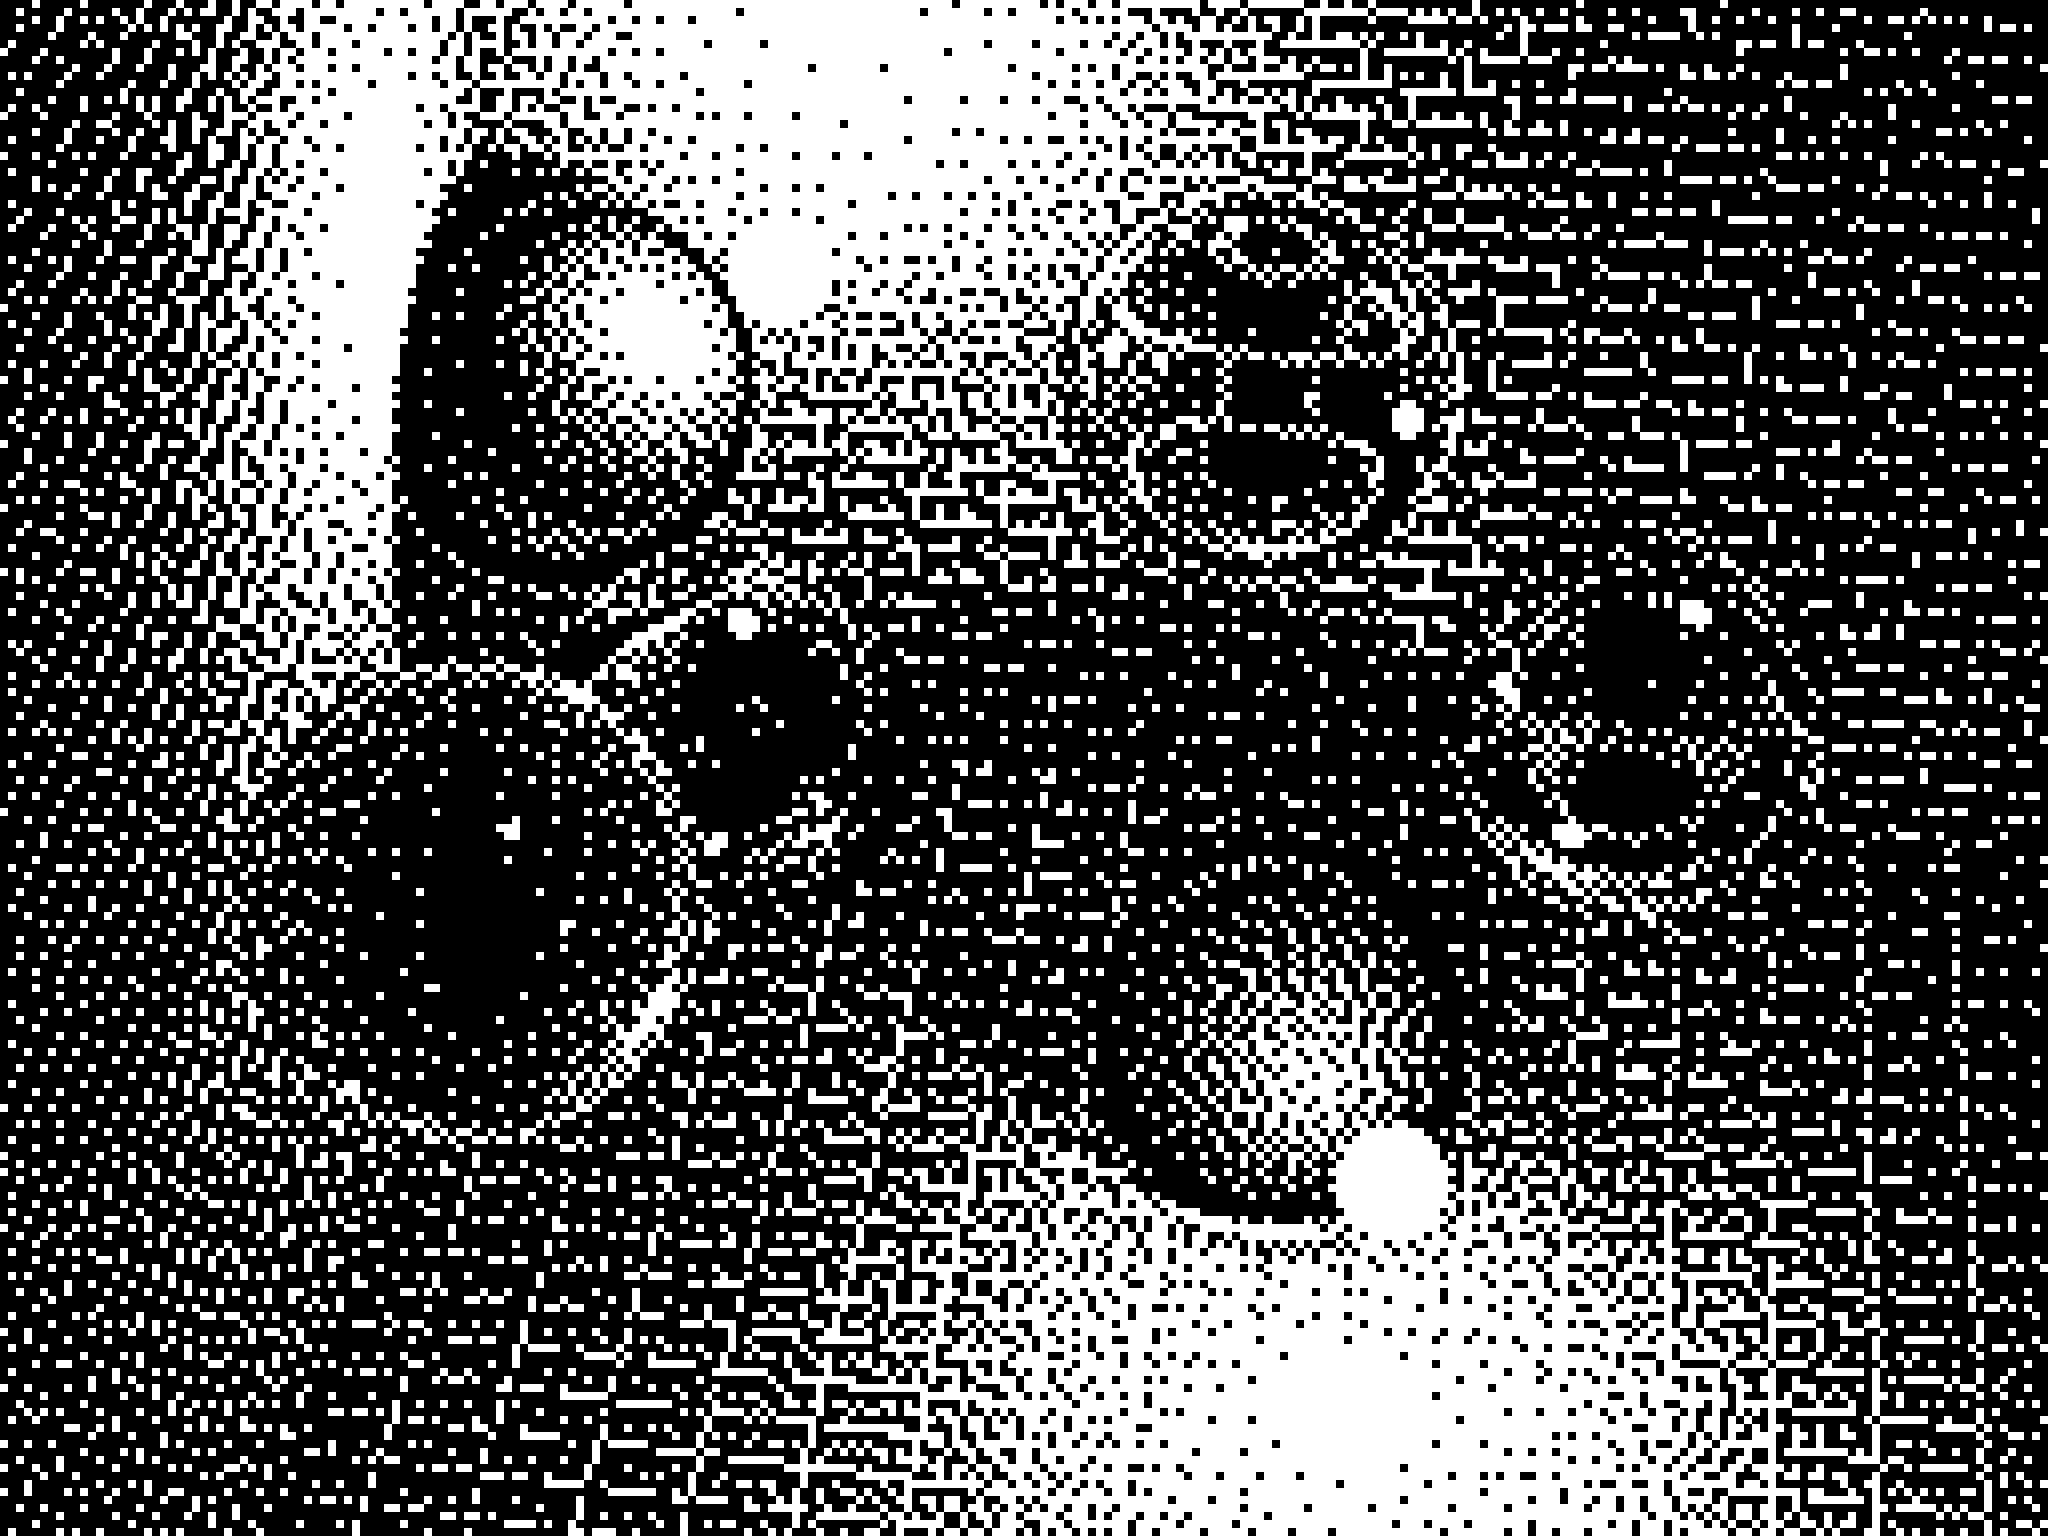
\includegraphics[width=1\textwidth]{logo.png}	\\
			\vspace{1cm}
			\Mail	\\
			\vspace{0.5cm}
			\textbf{\begin{LARGE} \Titolo \end{LARGE}}		\\
			\vspace{1cm}
			\textbf{Descrizione:} \Descrizione{}			\\
			\vspace{1cm}
			\begin{tabular}{ll}
				\textbf{Stato}               & \Stato              \\
				\textbf{Data}                & \Data               \\
				\midrule
				\textbf{Redattori}           & \Redattori          \\
				\textbf{Verificatori}        & \Verificatori       \\

				\ifdefined\Approvatori
				\textbf{Approvatori}         & \Approvatori        \\
				\fi

				\ifdefined\ApprovatoriInterni
				\textbf{Approvatori interni} & \ApprovatoriInterni \\
				\fi

				\ifdefined\ApprovatoriEsterni
				\textbf{Approvatori esterni} & \ApprovatoriEsterni \\
				\fi

				\ifdefined\Destinatari
				\textbf{Destinatari}         & \Destinatari        \\
				\fi

				\midrule

				\ifdefined\Versione
				\textbf{Versione}            & \Versione           \\
				\fi
			\end{tabular}
		\end{center}
		\vspace{4cm}
	\end{titlepage}
	\newpage
}

	\fancypagestyle{plain}{
	\fancyhf{}
	\rhead{ 
\includegraphics[scale=0.05]{horizontal_logo.png}}
	\lhead{\Titolo \ifdefined\Versione \ \Versione \fi}
	%\lfoot{\Titolo}
	\rfoot{\thepage{} di \pageref{LastPage}}
	\renewcommand{\headrulewidth}{0.2pt}
	\renewcommand{\footrulewidth}{0.2pt}
}
\pagestyle{plain}

	% ... altri template
\end{lstlisting}

In questo modo è possibile mantenere uniforme la struttura di tutti i
documenti e semplificarne la creazione.

\subsection{Variabili dei documenti}

Ciascun documento deve definire alcune variabili che sono utilizzate per
costruirne la struttura e la copertina. Di seguito sono elencate le variabili da
definire per ciascun documento:
\begin{itemize}
	\item \textbf{Verbale interno}:
	      \begin{itemize}
		      \item \textbf{Titolo}: "Verbale interno".
		      \item \textbf{Data}: la data in cui ha avuto luogo la riunione.
		      \item \textbf{Versione}: la versione del verbale.
		      \item \textbf{Descrizione}: una breve descrizione del verbale.
		      \item \textbf{\gls{Stato}$^G$}: lo \gls{Stato}$^G$ del verbale, ovvero se è \gls{Stato}$^G$
		            approvato o meno.
		      \item \textbf{Redattori}: i redattori del verbale (in genere è il
		            responsabile).
		      \item \textbf{Verificatori}: i verificatori del verbale (in genere
		            è il verificatore).
	      \end{itemize}

	\item \textbf{Verbale esterno}:
	      \begin{itemize}
		      \item \textbf{Titolo}: "Verbale esterno - Imola Informatica".
		      \item \textbf{Data}: la data in cui ha avuto luogo la riunione.
		      \item \textbf{Versione}: la versione del verbale;
		      \item \textbf{Descrizione}: una breve descrizione del verbale.
		      \item \textbf{\gls{Stato}$^G$}: lo \gls{Stato}$^G$ del verbale, ovvero se è \gls{Stato}$^G$
		            approvato o meno.
		      \item \textbf{Redattori}: i redattori del verbale (in genere è il
		            responsabile).
		      \item \textbf{Verificatori}: i verificatori del verbale (in genere
		            è il verificatore).
		      \item \textbf{Approvatori esterni}: i nomi degli approvatori
		            esterni, ovvero dei proponenti.
	      \end{itemize}

	      Nota bene, ciascun verbale esterno deve essere firmato dai proponenti,
	      per questo motivo è necessario inserire uno spazio apposito alla fine
	      del documento attraverso il comando \texttt{\\firma\{\}} definito nel
	      \textit{template} \texttt{firma.tex}.

	\item \textbf{Documenti generici}:
	      \begin{itemize}
		      \item \textbf{Titolo}: il nome del documento.
		      \item \textbf{Data}: la data di creazione del documento.
		      \item \textbf{Versione}: la versione del documento.
		      \item \textbf{Descrizione}: una breve descrizione del documento.
		      \item \textbf{\gls{Stato}$^G$}: lo \gls{Stato}$^G$ del documento, ovvero se è \gls{Stato}$^G$
		            approvato o meno.
	      \end{itemize}

\end{itemize}


\subsection{Versionamento}
\label{documentazione_versionamento}
Ogni documento rilasciato dovrà presentare un versionamento interno indicato con
tre interi positivi nel formato \texttt{X.Y.Z}, dove:
\begin{itemize}
	\item \textbf{X}: da incrementare in di rilascio di un
	      documento, indica l'ultima versione ufficialmente rilasciata.
	      L'incremento di questa cifra comporta l'azzeramento delle cifre Y e Z
	      e avviene con modalità differenti a seconda del documento.

	\item \textbf{Y}: da incrementare in caso avvenga la verifica e
	      l'approvazione di un documento; indica il numero di verifiche
	      effettuate sul documento. L'incremento di questa cifra comporta
	      l'azzeramento della cifra Z.

	\item \textbf{Z}: da incrementare in caso avvenga modifica, creazione o
	      eliminazione di una qualunque porzione di testo del documento; indica
	      il numero di modifiche effettuate sul documento.
\end{itemize}

Ogni documento dovrà essere creato partendo dalla versione \texttt{0.0.1}, ogni
s\gls{UC}$^G$cessivo incremento alla versione dovrà essere accompagnato da una nuova riga
nella tabella "Registro delle modifiche" che espliciti i cambiamenti effettuati.
Modifiche quali correzioni grammaticali o leggere variazioni nel testo non vanno
riportate nel registro delle modifiche e non prod\gls{UC}$^G$ono un avanzamento di
versione.
La verifica di un documento comporta l'incremento della cifra Y, mentre
L'approvazione di un documento avviene solo quando il documento deve essere
rilasciato.

\subsection{Verifica di un documento}
Ogni documento deve essere necessariamente verificato da un Verificatore, il
quale si occuperà di revisionare i seguenti aspetti:
\begin{itemize}
	\item Correttezza grammaticale.
	\item Correttezza logica.
	\item Correttezza e completezza del contenuto in modo che risulti coerente
	      con il documento.
	\item Adesione al \textit{Way of Working}.
\end{itemize}
\noindent
In caso il verificatore dovesse riscontrare dei problemi questi vanno segnalati
su \gls{\gls{Git}$^G$Hub} tramite i commenti presenti all'interno dell'apposita sezione
"Pull Request".
Questa azione genera una notifica immediata al red\gls{Attore}$^G$, il quale provvederà
ad apportare le modifiche necessarie. \\
In caso invece il documento non richieda modifiche si dovrà procedere ad un
avanzamento di versione come descritto in sezione
\S\ref{documentazione_versionamento}.


\subsection{Approvazione di un documento}
L'approvazione di un documento avviene solo quando il documento deve essere
rilasciato. A seconda del documento, l'approvazione interna è svolta in modo
diverso:
\begin{itemize}
	\item \textbf{Verbali}: un verbale viene approvato quando un verificatore
	      ritiene che il documento sia pronto per il rilascio.

	\item \textbf{Altri documenti}: l'incremento di questa cifra avviene
	      quando due verificatori ritengono che il documento sia pronto per il
	      rilascio.
\end{itemize}

Ogni documento approvato deve subire un avanzamento di versione come descritto
alla sezione \S\ref{documentazione_versionamento}.
\noindent
In caso il documento in questione sia un verbale esterno, il verificatore dovrà
occuparsi di effettuare una approvazione interna e, s\gls{UC}$^G$cessivamente, inviare il
documento in allegato ad una \textit{email} al fine di ottenere l'approvazione
esterna del verbale. Una volta firmato il documento, il verificatore dovrà
inserire il documento nella \textit{\gls{Repository}$^G$}
\href{https://\gls{\gls{Git}$^G$Hub}.com/Project-SWEnergy/Project-SWEnergy.\gls{\gls{Git}$^G$Hub}.io}{\texttt{Project-SWEnergy.\gls{\gls{Git}$^G$Hub}.io}}
nella cartella \texttt{verbali\_esterni}.


\subsection{Struttura dei verbali interni}

I verbali interni sono suddivisi in 4 porzioni, in \gls{Ordine}$^G$:
\begin{itemize}
	\item \textbf{\gls{Partecipanti}$^G$}: in questa sezione è indicata la durata della
	      riunione. Di seguito è presente una tabella che indica i nomi dei
	      componenti di SWEnergy, il loro ruolo e la durata della partecipazione
	      alla riunione.

	\item \textbf{\gls{Ordine}$^G$ del giorno}: in questa sezione è presente una lista
	      dei punti che sono stati discussi durante la riunione e le pagine nel
	      quale sono trattati. Si noti che questa sezione è generata
	      automaticamente e corrisponde alla tabella dei contenuti.

	\item \textbf{Sezioni di approfondimento}: sono presenti più sezioni che
	      spiegano ciascuno dei punti dell'\gls{Ordine}$^G$ del giorno. La prima di queste
	      sezioni deve essere il \textit{Brainstorming} che rappresenta il
	      resoconto delle attività svolte nell'ultimo mini-\textit{sprint}.

	\item \textbf{Assegnazione degli incarichi}: in questa sezione sono
	      presenti gli incarichi assegnati ai vari componenti del gruppo, viene
	      anche indicata la \textit{\gls{Issue}$^G$} di \gls{\gls{Git}$^G$Hub} di riferimento se presente.
\end{itemize}

\subsection{Struttura dei verbali esterni}
I verbali esterni hanno una struttura simile a quella dei verbali interni, ma
sono presenti alcune differenze:
\begin{itemize}
	\item \textbf{\gls{Partecipanti}$^G$}: in questa sezione è indicata la durata della
	      riunione. Di seguito è presente una tabella che indica i nomi dei
	      componenti di SWEnergy, il loro ruolo e la durata della partecipazione
	      alla riunione. In questa tabella viene anche inserito il nome dei
	      proponente presenti alla riunione.

	\item \textbf{\gls{Ordine}$^G$ del giorno}: questa sezione è identica a quella dei
	      verbali interni. Ovvero, è presente una lista dei punti che sono stati
	      trattati durante il \textit{meeting} e le pagine nel quale sono
	      approfonditi gli argomenti. Questa pagina è generata automaticamente
	      e corrisponde alla tabella dei contenuti.

	\item \textbf{Sezioni di approfondimento}: questa sezione è identica a
	      quella dei verbali interni. Ovvero, sono presenti più sezioni che
	      spiegano ciascuno dei punti dell'\gls{Ordine}$^G$ del giorno. La prima di queste
	      sezioni deve essere il \textit{Brainstorming} che rappresenta il
	      resoconto delle attività svolte nell'ultimo mini-\textit{sprint}.

	\item \textbf{Conclusioni}: in questa sezione sono presenti le conclusioni
	      del \textit{meeting} e le decisioni prese. In particolare, in questa
	      sezione sono chiariti gli impegni presi dal gruppo che dovranno essere
	      risolti entro la prossima riunione.
\end{itemize}

\subsection{Struttura dei documenti generici}

Poiché i documenti generici sono molto diversi tra loro e sono unici, non è
trattata la descrizione della loro struttura. Piuttosto, si richiede che in ogni
documento sia presente un'introduzione che ne descriva lo scopo e la struttura.
Di seguito sono riportati gli elementi comuni a tutti i documenti generici che
devono essere presenti:
\begin{itemize}
	\item \textbf{Registro delle modifiche}:
	      Ogni documento, esclusi verbali e presentazione, include subito dopo
	      la copertina un registro delle modifiche in forma tabellare, come
	      indicato nei riferimenti. Vi sono le seguenti voci:
	      \begin{itemize}
		      \item \textbf{Versione}: indica da versione del documento alla
		            riga di modifica.
		      \item \textbf{Data}: indica la data di redazione, verifica o
		            approvazione.
		      \item \textbf{Red\gls{Attore}$^G$}: nome del componente del gruppo che ha
		            effettuato la redazione.
		      \item \textbf{Verificatore}: nome del componente del gruppo che ha
		            effettuato la verifica.
		      \item \textbf{Approvatore}: nome del componente del gruppo che ha
		            effettuato l'approvazione.
		      \item \textbf{Descrizione}: breve descrizione della sezione
		            oggetto di redazione e verifica, in caso di approvazione
		            indica l'azione svolta e la fase di avanzamento attuale.
	      \end{itemize}
	      \noindent
	      La tabella viene riportata in \gls{Ordine}$^G$ decrescente di modifica, così da
	      mantenere sempre in cima le azioni più recenti eseguite.

	\item \textbf{Indice}:
	      Ogni documento include subito dopo il registro delle modifiche un
	      indice che elenca le sezioni del documento. L'indice è generato
	      automaticamente e corrisponde alla tabella dei contenuti.

	\item \textbf{Introduzione}:
	      Ogni documento include, subito dopo l'indice, un'introduzione che
	      descrive lo scopo del documento e la struttura del documento stesso.
	      Ciascuna introduzione deve contenere le seguenti sotto-sezioni:
	      \begin{itemize}
		      \item \textbf{Scopo del documento}: descrive lo scopo del
		            documento.
		      \item \textbf{Scopo del prodotto}: descrive lo scopo del prodotto
		            che si andrà a realizzare.
		      \item \textbf{Glossario}: contiene i termini che necessitano di
		            ulteriore contestualizzazione o che necessitano di essere
		            chiariti.
		      \item \textbf{Riferimenti}: contiene i riferimenti utilizzati
		            durante la stesura del documento, sia interni che esterni.
	      \end{itemize}
\end{itemize}

\subsection{Diario di bordo}

Il diario di bordo è una presentazione \textit{PowerPoint} che viene mostrata
al committente ad intervalli regolari. I diari di bordo si trovano nella
cartella \texttt{diario\_di\_bordo} su \textit{Google Drive}, nell'account del
gruppo SWEnergy.

\subsection{Creazione del diario di bordo}

Per creare il diario di bordo è necessario seguire i seguenti passi:
\begin{enumerate}
	\item Si visualizza un diario di bordo precedente.
	\item Si effettua una copia del diario di bordo precedente.
	\item Si aggiorna la prima diapositiva con le informazioni della nuova
	      riunione.
	\item Si aggiornano gli header con la data della nuova riunione.
	\item Si aggiorna la seconda diapositiva con le attività svolte e i problemi
	      riscontrati.
	\item Si aggiorna la terza diapositiva con le attività da svolgere e i dubbi
	      inerenti.
\end{enumerate}

In ogni caso, il diario di bordo deve essere creato in una riunione di gruppo
precedente alla riunione con il committente. In particolare, il diario di bordo
deve essere creato in seguito alla retrospettiva del mini-\textit{sprint}.

\subsubsection{Struttura del diario di bordo}

In ciascuna diapositiva devono essere presenti
\begin{itemize}
	\item \textbf{Logo}: il logo del gruppo in basso a sinistra.
	\item \textbf{Numero diapositiva}: il numero della diapositiva in basso a
	      destra rispetto al numero totale di diapositive.
	\item \textbf{\textit{Header}}: ":\textbackslash{}Università
	      degli Studi di Padova\textbackslash{}Diario di bordo\textbackslash{}"
	      più la data della riunione nel formato "GG\_MM\_AAAA".
\end{itemize}

Ogni diario di bordo è composto da 4 diapositive, in \gls{Ordine}$^G$:
\begin{enumerate}
	\item \textbf{Introduzione}: contiene il logo del gruppo e il nome del
	      gruppo. In aggiunta, contiene il nome del documento, la città in cui è
	      tenuta la riunione e la data della riunione.

	\item \textbf{Brainstorming}: contiene il resoconto delle attività svolte
	      dall'ultimo diario di bordo e i problemi riscontrati duranto lo
	      svolgimento delle attività.

	\item \textbf{Pianificazione}: contiene la pianificazione delle attività
	      da svolgere fino al prossimo diario di bordo. In particolare, sono
	      presenti le attività da svolgere e i dubbi da chiarire prima di poter
	      affrontare le attività.

	\item \textbf{Chi siamo}: contiene una breve descrizione dei componenti
	      del gruppo.
\end{enumerate}


\subsection{Gestione della Configurazione}

La gestione della configurazione è un processo di supporto che assicura il
controllo delle versioni e la tracciabilità dei componenti \textit{software}
durante tutto il ciclo di vita del progetto.
Questo processo si occupa di mantenere la coerenza delle prestazioni, dei dati
funzionali e delle informazioni fisiche di un sistema e dei suoi componenti.
Si focalizza sulla gestione di modifiche e configurazioni per prevenire
disordine e confusione.

\subsubsection{Scopo}
Questo processo ha lo scopo di assicurare che tutti i componenti del
\textit{software} siano identificati, versionati e tracciati nel corso del
tempo, facilitando così la gestione delle modifiche e migliorando la qualità
del prodotto \textit{software}.

\subsubsection{Attività}
\begin{enumerate}
	\item \textbf{Identificazione della configurazione:} Definire e documentare
	      le caratteristiche funzionali e fisiche dei componenti
	      \textit{software}.
	\item \textbf{Controllo della configurazione:} Gestire le modifiche
	      attraverso un processo formale di valutazione, approvazione e
	      implementazione.
	\item \textbf{Registrazione e rapporto dello stato di configurazione:}
	      Tenere traccia di tutte le modifiche apportate ai componenti
	      \textit{software} e documentare lo stato corrente di configurazione.
	\item \textbf{Verifica:} Assicurare che i componenti \textit{software} siano
	      conformi ai requisiti e che le modifiche siano implementate
	      correttamente.
\end{enumerate}

\subsubsection{Strumenti}
\begin{itemize}
	\item \textbf{Git}: Sistema di controllo versione distribuito utilizzato per
	      il tracciamento delle modifiche al codice sorgente;
	\item \textbf{GitHub\g}: Piattaforma di \textit{hosting} per progetti \textit{software}
	      che fornisce strumenti di collaborazione e controllo versione e
	      traccia delle \textit{issue\g};
	\item \textbf{GitHub Actions}: Strumento di automazione per l'esecuzione di
	      \textit{workflow} personalizzati.
\end{itemize}

\subsection{Accertamento della Qualità}

L'accertamento della qualità è un processo di supporto fondamentale che
garantisce che il \textit{software} soddisfi i requisiti di qualità stabiliti e
le aspettative degli \textit{stakeholder}.
Questo processo include la definizione, implementazione, valutazione e
manutenzione delle procedure e delle politiche di qualità per assicurare che
il \textit{software} prodotto sia di alta qualità.

\subsubsection{Scopo}
Assicurare che il \textit{software} e le pratiche di sviluppo rispettino gli
standard di qualità prefissati, migliorando così la soddisfazione del cliente e
l'affidabilità del prodotto.

\subsubsection{Attività}
\begin{enumerate}
	\item \textbf{Definizione delle Politiche di Qualità:} Stabilire gli
	      standard e le metriche di qualità in base ai requisiti del progetto e
	      alle aspettative degli \textit{stakeholder}.
	\item \textbf{Implementazione delle Procedure di Qualità:} Applicare le
	      politiche attraverso metodi concreti e pratiche di sviluppo, come
	      revisioni del codice e test.
	\item \textbf{Valutazione della Conformità:} Verificare periodicamente che
	      il \textit{software} e i processi di sviluppo rispettino le politiche
	      di qualità stabilite.
	\item \textbf{Manutenzione e Miglioramento Continuo:} Aggiornare le
	      politiche e le procedure di qualità in base ai \textit{feedback\g} e ai
	      risultati delle valutazioni per promuovere il miglioramento continuo
	      (vedi \autoref{aggiornare-pdq}).
\end{enumerate}

\subsubsection{Strumenti}
Gli strumenti utilizzati nel processo di accertamento della qualità possono
includere \textit{software} autoprodotti di automazione dei test e di raccolta
dei dati.

\section{Attività di verifica}
Si analizzano qui le metriche:
\begin{itemize}
    \item \hyperref[s:mpc02]{\textbf{MPC02}}\textbf{}: \textit{Budget Variance}.
    \item \hyperref[s:mpc04]{\textbf{MPC04}}\textbf{}: \textit{Budgeted Cost of Work Scheduled}.
    \item \hyperref[s:mpc06]{\textbf{MPC06}}\textbf{}: \textit{Actual Cost of Work Performed}.
    \item \hyperref[s:mpc07]{\textbf{MPC07}}\textbf{}: \textit{Requirements stability index}.
    \item \hyperref[s:mpc08]{\textbf{MPC08}}\textbf{}: \textit{Satisfied obligatory requirements}.
    \item \hyperref[s:mpc09]{\textbf{MPC09}}\textbf{}: \textit{Non-calculated risk}.
    \item \hyperref[s:mpc10]{\textbf{MPC10}}\textbf{}: \textit{Code Coverage}.
    \item \hyperref[s:mpc11]{\textbf{MPC11}}\textbf{}: \textit{Passed Test Cases Percentage}.
    \item \hyperref[s:mpd1]{\textbf{MPD1}}\textbf{}: Indice di Gulpease.
    \item \hyperref[s:mpd2]{\textbf{MPD2}}\textbf{}: Copertura dei requisiti.
    \item \hyperref[s:mpd9]{\textbf{MPD9}}\textbf{}: Browser supportati.

\end{itemize}
\newpage


\subsection{MPC02 - Budget Variance}
\label{s:mpc02}
La \textit{Budget Variance} confronta il costo effettivo del lavoro completato fino a un certo punto nel tempo con il costo pianificato per quel lavoro.
Il valore negativo riportato in Figura \ref{fig:mpc02} indica che il costo effettivo è superiore al \textit{budget} pianificato.
Il valore medio riportato rientra nel margine di accettabilità stabilito. \\
Il gruppo ritiene che, nella prima fase RTB, lo sforamento del \textit{budget} sia dovuto alla generale inesperienza dei vari membri nella gestione di un progetto e nell'uso delle tecnologie, che ha portato alla necessità di incrementare il tempo di lavoro.\\
Nella seconda fase il gruppo ha individuato delle problematiche che non erano note nella fase precedente, questo grazie all'esperienza maturata durante lo sviluppo.
Tali problematiche hanno aumentato le attività da svolgere per mettere in atto operazioni di correzione, questo ha portato ad uno sforamento del \textit{budget}.
In particolare durante il sesto \textit{sprint}, il gruppo si è reso conto di aver sottostimato le ore necessarie per svolgere le attività di programmazione.
La pianificazione delle attività negli \textit{sprint} successivi è stata quindi rivista adeguando le ore necessarie alla programmazione con quandto sperimentato nello \textit{sprint} numero 6.

\begin{figure}[ht]
    \centering
    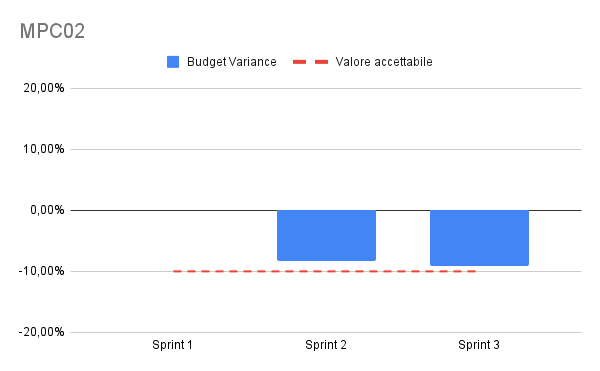
\includegraphics[width=0.8\textwidth]{img/MPC02.png}
    \caption{MPC02 - Budget Variance}
    \label{fig:mpc02}
\end{figure}

\newpage


\subsection{MPC04 - Budgeted Cost of Work Scheduled}
\label{s:mpc04}
Rappresenta il costo del lavoro pianificato per essere completato entro una data specifica nel progetto.\\
Nel grafico in Figura \ref{fig:mpc04} è stato inserito anche il costo relativo ad ogni \textit{sprint} al fine di indicare più intuitivamente il contributo di ogni singola fase al costo complessivo.\\
Il minor costo associato al quarto \textit{sprint} deriva dalla necessità di ridurre le ore di lavoro utile in concomitanza dei numerosi impegni, sia personali che legati alla sessione di esami, dei membri del gruppo.\\
Il consumo di risorse, confrontato con il preventivo dei costi presente nel documento \href{https://project-swenergy.github.io/Candidatura/Presentazione%20costi%20e%20assunzione%20impegni.pdf}{Presentazione costi ed assunzione impegni v2.0.0}, risulta ragionevole in considerazione della diversa durata delle fasi RTB e PB.\\
A partire dalla fase PB, relativa allo \textit{sprint} numero 5, si ha una crescita lineare costante che indica:
\begin{itemize}
    \item \textbf{Stima accurata}: le stime iniziali per il progetto sono precise e il lavoro si sta svolgendo secondo la pianificazione senza grandi variazioni o imprevisti.
    \item \textbf{Stabilità del processo}: indica che il processo utilizzato per completare il lavoro è stabile e prevedibile.
    \item \textbf{Controllo del progetto}: indica che il progetto è ben gestito e che ci sono processi di controllo efficaci per monitorare il progresso e intervenire tempestivamente in caso di deviazioni dalla pianificazione.
\end{itemize}
\vspace{1.5em}
Le problematiche riscontrate durante lo sviluppo sono quindi state correttamente gestite per consentire un progresso lineare e, quindi, più facilmente gestibile.
\begin{figure}[h]
    \centering
    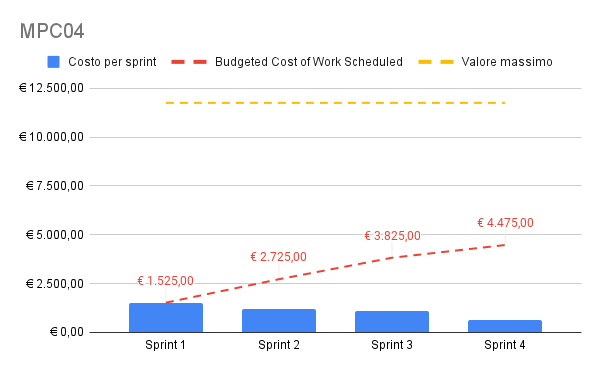
\includegraphics[width=0.8\textwidth]{img/MPC04.png}
    \caption{MPC04 - Budgeted Cost of Work Scheduled}
    \label{fig:mpc04}
\end{figure}


\subsection{MPC06 - Actual Cost of Work Performed}
\label{s:mpc06}
Il valore riportato in Figura \ref{fig:mpc06} indica che, a seguito del primo \textit{sprint}, il costo effettivo sostenuto ha superato quello preventivato.\\
Il gruppo ritiene che che il superamento del costo preventivato sia dovuto alla generale inesperienza dei vari membri nella gestione di un progetto e nell'uso delle tecnologie, che ha portato alla necessità di incrementare il tempo di lavoro nella fase iniziale del progetto.\\
Nonostante il superamento del valore ottimale, il costo effettivo è rimasto complessivamente all'interno del margine di accettabilità indicato nella metrica in esame.

\begin{figure}[htbp]
    \centering
    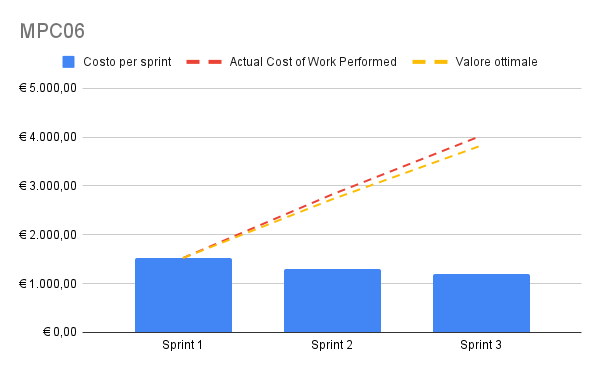
\includegraphics[width=0.7\textwidth]{img/MPC06.png}
    \caption{MPC06 - Actual Cost of Work Performed}
    \label{fig:mpc06}
\end{figure}


\subsection{MPC07 - Requirements stability index}
\label{s:mpc07}
Indica la stabilità dei requisiti nel corso del tempo.
Un RSI più alto indica una maggiore instabilità dei requisiti, mentre un RSI più basso indica una maggiore stabilità.
I requisiti sono stati aggiornati in seguito alla fase RTB, a seguito del dialogo con il proponente e alla presentazione del lavoro svolto.
Le modifiche apportate ai requisiti rientrano comunque all'interno del margine di accettabilità previsto.
\begin{table}[H]
    \centering
    \begin{tabularx}{\textwidth}{X|l|l|l|l}
        \hline
        \textbf{Metrica}             & \textbf{Codice} & \textbf{Valore ottimale} & \textbf{Valore accettabile} & \textbf{Valore attuale} \\
        \hline
        Requirements stability index & MPC07           & 0\%                      & 10\%                        & 8\%                     \\
        \hline
    \end{tabularx}
\end{table}


\subsection{MPC08 - Satisfied obligatory requirements}
\label{s:mpc08}
Il numero di requisiti obbligatori è stato ridotto a seguito del colloquio avuto con il proponente nell'ottavo \textit{sprint}.
La necessità di ridurre il numero di requisiti obbligatori è stata causata dal ritardo accumulato nello sviluppo e dalla necessità di mantenere il più possibile invariata la data di consegna del progetto.
Al termine del nono \textit{sprint} sono stati soddisfatti tutti i requisiti obbligatori individuati.
\begin{table}[H]
    \centering
    \begin{tabularx}{\textwidth}{X|l|l|l|l}
        \hline
        \textbf{Metrica}                  & \textbf{Codice} & \textbf{Valore ottimale} & \textbf{Valore accettabile} & \textbf{Valore attuale} \\
        \hline
        Satisfied obligatory requirements & MPC08           & 100\%                    & 100\%                       & 100\%                   \\
        \hline
    \end{tabularx}
\end{table}


\subsection{MPC09 - Non-calculated risk}
\label{s:mpc09}
Questa metrica si riferisce ai rischi che non sono stati attentamente valutati o considerati durante lo sviluppo del software.
Durante lo sviluppo del progetto i rischi sono stati valutati correttamente e sono state previste procedure per la mitigazione.
Le informazioni inerenti i rischi individuati dal gruppo sono visibili nel documento "Piano di Progetto v2.0.0".
\begin{table}[H]
    \centering
    \begin{tabularx}{\textwidth}{X|l|l|l|l}
        \hline
        \textbf{Metrica}    & \textbf{Codice} & \textbf{Valore ottimale} & \textbf{Valore accettabile} & \textbf{Valore attuale} \\
        \hline
        Non-calculated risk & MPC09           & 0                        & 5                           & 0                       \\
        \hline
    \end{tabularx}
\end{table}


\subsection{MPC10 - Code Coverage}
\label{s:mpc10}
Sono state valutate quattro misure inerenti la copertura del codice tramite test di unità.
Vengono qui riportate divise tra il gruppo dedicatosi al \textit{frontend} e quello dedicatosi al \textit{backend}.
Insieme alla metrica MPC11 fornisce una panoramica della qualità del codice.
\begin{table}[H]
    \centering
    \begin{tabularx}{\textwidth}{X|l|l|l|l}
        \hline
        \textbf{Metrica}    & \textbf{Codice} & \textbf{Valore ottimale} & \textbf{Valore accettabile} & \textbf{Valore attuale} \\
        \hline
        \textit{Statements} & MPC10           & $100\%$                  & $\ge 80\%$                  & $ 92\%$                 \\
        \hline
        \textit{Branches}   & MPC10           & $100\%$                  & $\ge 80\%$                  & $ 86\%$                 \\
        \hline
        \textit{Functions}  & MPC10           & $100\%$                  & $\ge 80\%$                  & $ 93\%$                 \\
        \hline
        \textit{Lines}      & MPC10           & $100\%$                  & $\ge 80\%$                  & $ 92\%$                 \\
        \hline
    \end{tabularx}
    \caption{\textit{Code coverage Frontend}}
\end{table}
\begin{table}[H]
    \centering
    \begin{tabularx}{\textwidth}{X|l|l|l|l}
        \hline
        \textbf{Metrica}    & \textbf{Codice} & \textbf{Valore ottimale} & \textbf{Valore accettabile} & \textbf{Valore attuale} \\
        \hline
        \textit{Statements} & MPC10           & $100\%$                  & $\ge 80\%$                  & $ 90\%$                 \\
        \hline
        \textit{Branches}   & MPC10           & $100\%$                  & $\ge 80\%$                  & $ 87\%$                 \\
        \hline
        \textit{Functions}  & MPC10           & $100\%$                  & $\ge 80\%$                  & $ 93\%$                 \\
        \hline
        \textit{Lines}      & MPC10           & $100\%$                  & $\ge 80\%$                  & $ 89\%$                 \\
        \hline
    \end{tabularx}
    \caption{\textit{Code coverage Backend}}
\end{table}


\subsection{MPC11 - Passed Test Cases Percentage}
Questo valore indica quanto sia riuscito il processo di testing rispetto al numero totale di casi di test eseguiti.
Insieme alla metrica MPC10 fornisce una panoramica della qualità del codice.

\label{s:mpc11}
\begin{table}[H]
    \centering
    \begin{tabularx}{\textwidth}{X|l|l|l|l}
        \hline
        \textbf{Metrica}     & \textbf{Codice} & \textbf{Valore ottimale} & \textbf{Valore accettabile} & \textbf{Valore attuale} \\
        \hline
        Passed Test Frontend & MPC11           & $100\%$                  & $ 100\%$                    & $ 100\%$ (414)          \\
        \hline
        Passed Test Backend  & MPC11           & $100\%$                  & $ 100\%$                    & $ 100\%$ (458)          \\
        \hline
    \end{tabularx}
\end{table}


\subsection{MPD1 - Indice di Gulpease}
\label{s:mpd1}
Il grafico in Figura \ref{fig:mpd1} mostra un miglioramento nella leggibilità media dei documenti redatti, avvenuto a seguito della fase di Candidatura.\\
Questo miglioramento è dovuto alla definizione di metriche di qualità che hanno portato il gruppo a prestare maggiore attenzione durante la scrittura della documentazione.
Il valore medio dell'indice di Gulpease ha così superato, per la fase RTB, la soglia di accettabilità.

\begin{figure}[htbp]
    \centering
    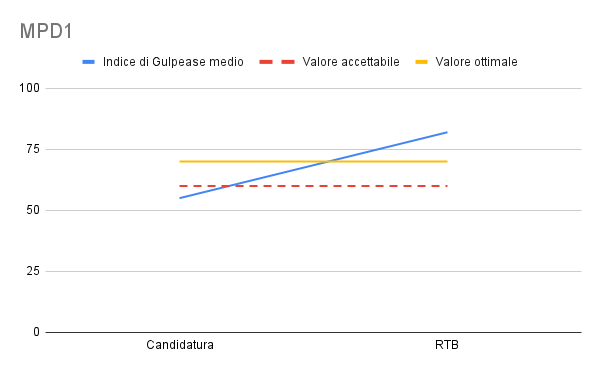
\includegraphics[width=0.7\textwidth]{img/MPD1.png}
    \caption{MPD1 - Indice di Gulpease}
    \label{fig:mpd1}
\end{figure}


\subsection{MPD2 - Copertura dei requisiti}
Non è stato possibile raggiungere il valore ottimale di copertura dei requisiti.\\
Durante la fase PB il gruppo si è reso conto, approfondendo la conoscenza delle tecnologie utilizzate, di aver sottostimato il tempo necessario per l'implementazione delle funzionalità previste all'inizio del progetto.
Questo ha portato ad una ristrutturazione del documento Analisi dei requisiti, riducendo il numero di requisiti obbligatori presenti.
Siccome le ore di lavoro disponibili sono rapidamente state consumate per le attività di codifica, il gruppo ha scelto di non soddisfare parte dei requisiti non obbligatori, preferendo non ritardare la data di consegna del progetto.
\label{s:mpd2}
\begin{table}[H]
    \centering
    \begin{tabularx}{\textwidth}{X|X|l|l|l}
        \hline
        \textbf{Metrica}        & \textbf{Codice} & \textbf{Valore ottimale} & \textbf{Valore accettabile} & \textbf{Valore attuale} \\
        \hline
        Copertura dei requisiti & MPD2            & $100\%$                  & $80\%$                      & $71\%$                \\
        \hline
    \end{tabularx}
\end{table}


\subsection{MPD9 - Browser supportati}
\label{s:mpd9}
Sono stati eseguiti test per verificare il corretto funzionamento dell'applicativo sui seguenti \textit{browser}:
\begin{itemize}
    \item Google Chrome
    \item Arc
    \item Opera GX
    \item Firefox
    \item Safari
    \item Microsfot Edge
\end{itemize}

\begin{table}[H]
    \centering
    \begin{tabularx}{\textwidth}{X|X|l|l|l}
        \hline
        \textbf{Metrica}   & \textbf{Codice} & \textbf{Valore ottimale} & \textbf{Valore accettabile} & \textbf{Valore attuale} \\
        \hline
        Browser supportati & MPD9            & $100\%$                  & $80\%$                      & $100\%$ (6)               \\
        \hline
    \end{tabularx}
\end{table}

\subsection{Approvazione}
\label{subsec:approvazione}

Il processo di approvazione si concentra sulla conferma che i requisiti e il
sistema \textit{software} o prodotto finito soddisfino il loro uso inteso
specifico. L'approvazione può essere condotta in fasi precedenti dello sviluppo.

\subsubsection{Scopo}

Questo processo assicura che il sistema \textit{software} o il prodotto finito
siano adeguatamente validati rispetto al loro uso previsto, contribuendo
significativamente all'affidabilità e alla soddisfazione dell'utente finale.

\subsubsection{Attività}
L'implementazione del processo di approvazione include le seguenti attività
principali:

\subsubsubsection{Identificazione} 
Valutare se il progetto richieda uno sforzo
	  di approvazione e il grado di indipendenza organizzativa di tale
	  sforzo.

\subsubsubsection{Pianificazione} 
Stabilire un processo di approvazione per
	  validare il sistema o il prodotto \textit{software} se il progetto lo
	  richiede. Selezionare i compiti di approvazione, inclusi i metodi, le
	  tecniche e gli strumenti associati.

\subsubsubsection{Approvare un documento}
\label{approvazione-documento}

\subsubsubsubsection{\textit{Trigger}}
\begin{itemize}
	\item Un documento viene completato rispetto alla fase attuale del progetto.
\end{itemize}

\subsubsubsubsection{Scopo}
\begin{itemize}
	\item Assicurarsi che il documento soddisfi i requisiti ad esso associati;

	\item Convalidare il contenuto ed il completameto del documento.
\end{itemize}

\subsubsubsubsection{Svolgimento}
\begin{itemize}
	\item \textbf{Approvazione:}
	      \begin{enumerate}
		      \item \textbf{Lettura}: il responsabile legge il
		            documento (vedi \cref{verifica-documento});

		      \item \textbf{Convalida}: il responsabile verifica che il
		            documento soddisfi i requisiti ad esso associati;

		      \item \textbf{Aggiornamento della versione}: dopo che il documento
		            viene corretto dall'autore, il responsabile aggiorna la
		            sua versione ed il suo stato;

		      \item \textbf{Versione}: sia $X.Y.Z$ la versione del documento,
		            dopo l'approvazione, il valore di $X$ viene incrementato di
		            $1$, mentre $Y$ e $Z$ vengono azzerati.
	      \end{enumerate}
\end{itemize}


\subsubsubsection{Rapporti} 
Inoltrare i rapporti di approvazione al committente e al proponente.

\subsection{Revisioni Congiunte con il Cliente}

Le revisioni congiunte con il cliente sono incontri strutturati tra il team di
sviluppo e gli \textit{stakeholder} o i clienti per esaminare il progresso del
prodotto \textit{software}, discutere problemi e trovare soluzioni congiunte.

\subsubsection{Scopo}
L'obiettivo di queste revisioni è assicurare che il prodotto \textit{software}
in sviluppo rispecchi fedelmente i requisiti e le aspettative del committente e
del proponente, e che eventuali discrepanze o incomprensioni siano risolte
tempestivamente.

\subsubsection{Attività}
\begin{enumerate}
	\item \textbf{Preparazione della Revisione:} Organizzare l'incontro,
	      definire l'agenda e preparare il materiale da presentare al
	      committente o al proponente (vedi
	      \autoref{organizzare-meeting-esterno}).
	\item \textbf{Conduzione della Revisione:} Presentare il lavoro svolto,
	      discutere i progressi e raccogliere \textit{feedback} dagli
	      \textit{stakeholder}.
	\item \textbf{Riscontro ai Feedback:} Analizzare e discutere i
	      \textit{feedback} ricevuti per determinare le azioni correttive
	      necessarie.
	\item \textbf{Pianificazione delle Azioni Correttive:} Definire un piano per
	      implementare le modifiche richieste o per risolvere problemi
	      identificati durante la revisione (vedi
	      \autoref{pianificazione-attivia}).
	\item \textbf{\textit{Follow-up}:} Monitorare l'attuazione delle azioni
	      correttive e organizzare revisioni successive se necessario.
\end{enumerate}

\subsubsection{Partecipanti}
Includono membri del team di sviluppo, rappresentanti del cliente o degli
\textit{stakeholder}, e possono includere anche esperti di dominio o utenti
finali.

\subsubsection{Documentazione}
Tutti gli aspetti salienti della revisione, compresi i \textit{feedback}, le
decisioni prese e le azioni correttive pianificate, devono essere documentati
all'interno dei verbali esterni e resi disponibili a tutti i partecipanti per
riferimento futuro.

\subsection{Verifiche Ispettive Interne}

Le verifiche ispettive interne sono processi attraverso i quali il team di
progetto esegue revisioni sistematiche e ispezioni dei propri processi e
prodotti \textit{software}, al fine di identificare e correggere gli errori
prima che il prodotto sia rilasciato o passi alla fase successiva.

\subsubsection{Scopo}
L'obiettivo delle verifiche ispettive interne è migliorare la qualità dei
processi e dei prodotti \textit{software}, riducendo gli errori, aumentando
l'efficienza e garantendo la conformità agli standard di progetto.

\subsubsection{Attività}
Le attività tipiche coinvolte nelle verifiche ispettive interne includono:

\begin{enumerate}
	\item \textbf{Pianificazione delle Ispezioni:} Definire gli obiettivi, lo
	      scopo, la portata e il programma delle ispezioni.
	\item \textbf{Preparazione:} Raccogliere e rivedere i documenti, il codice e
	      altri artefatti da ispezionare.
	\item \textbf{Conduzione delle Ispezioni:} Eseguire le ispezioni secondo le
	      procedure stabilite, utilizzando \textit{checklist} o linee guida
	      specifiche per identificare gli errori e le aree di miglioramento.
	\item \textbf{Riunione di Ispezione:} Discutere i risultati delle ispezioni
	      con il team, identificare le cause degli errori e decidere le azioni
	      correttive.
	\item \textbf{Implementazione delle Azioni Correttive:} Apportare le
	      modifiche necessarie per risolvere gli errori identificati durante le
	      ispezioni.
	\item \textbf{\textit{Follow-up}:} Verificare che tutte le azioni
	      correttive siano state implementate correttamente e che gli errori
	      siano stati risolti.
\end{enumerate}

\subsubsection{Partecipanti}
Le verifiche ispettive interne coinvolgono diversi ruoli all'interno del team
di progetto, tra cui verificatori, analisti, progettisti e programmatori,
ciascuno con responsabilità specifiche nel processo di ispezione.

\subsubsection{Documentazione}
Tutti i risultati delle ispezioni, comprese le scoperte, le decisioni prese e
le azioni correttive pianificate, devono essere documentati e archiviati per
future referenze e valutazioni della qualità.

\subsection{Risoluzione dei Problemi}

La risoluzione dei problemi si occupa della gestione sistematica dei problemi
riscontrati nel \textit{software} o nei processi di sviluppo, dalla loro
identificazione alla loro risoluzione e documentazione.

\subsubsection{Scopo}
Identificare e risolvere i problemi in modo efficiente per minimizzare l'impatto
sul progetto, migliorando la qualità del prodotto e del processo.

\subsubsection{Attività}
\begin{enumerate}
	\item \textbf{Identificazione del Problema:} Riconoscere e documentare i
	      problemi o le discrepanze riscontrate nel \textit{software} o nei
	      processi.
	\item \textbf{Analisi del Problema:} Valutare il problema per comprenderne
	      le cause radice e determinare l'impatto sul progetto.
	\item \textbf{Pianificazione delle Azioni Correttive:} Sviluppare un piano
	      di azioni per risolvere il problema, includendo modifiche al
	      \textit{software} o ai processi.
	\item \textbf{Implementazione delle Azioni Correttive:} Applicare le
	      soluzioni identificate per correggere il problema.
	\item \textbf{Verifica e Chiusura:} Verificare che la soluzione abbia
	      risolto efficacemente il problema e documentare l'esito e le lezioni
	      apprese.
\end{enumerate}

\subsubsection{Documentazione}
Documentare ogni problema riscontrato, le azioni intraprese per risolverlo e i
risultati ottenuti, per mantenere una tracciabilità e fornire un riferimento
per problemi futuri.

\subsubsection{Strumenti}
\begin{itemize}
	\item \textbf{\textit{Discussion} di GitHub\g}: Strumento per la gestione ed
	      il mantenimento di discussioni su problemi e soluzioni.
\end{itemize}


\section{Processi Organizzativi}
\label{sec:processi_organizzativi}

I processi organizzativi sono fondamentali per garantire l'efficienza e l'
efficacia dei processi di ciclo di vita del \textit{software} all'interno dell'
organizzazione del progetto. Essi forniscono supporto trasversale a tutti i
progetti e contribuiscono alla gestione delle risorse, al miglioramento
continuo e alla formazione del personale.

\subsection{Gestione dei Processi}

La gestione dei processi comprende le attività di pianificazione, monitoraggio
e controllo dei processi di ciclo di vita del \textit{software} all'interno del
progetto, assicurando che siano condotti in modo efficace ed efficiente.

\subsubsection{Scopo}
Il principale obiettivo della gestione dei processi è migliorare la qualità
del \textit{software} prodotto e l'efficienza dello sviluppo, attraverso la
standardizzazione dei processi e l'implementazione delle migliori pratiche.

\subsubsection{Attività}
\begin{enumerate}
	\item \textbf{Pianificazione dei Processi:} Definire gli obiettivi, le
	      procedure e i piani per l'esecuzione e il controllo dei processi di
	      ciclo di vita del \textit{software} (vedi
	      \cref{pianificazione-attivia} e \cref{aggiornare-pdp}).
	\item \textbf{Monitoraggio e Controllo:} Tenere traccia dei progressi
	      rispetto ai piani stabiliti e intervenire in caso di deviazioni, per
	      assicurare l'allineamento con gli obiettivi di progetto.
	\item \textbf{Valutazione dei Processi:} Analizzare periodicamente
	      l'efficacia e l'efficienza dei processi attuati, identificando aree di
	      miglioramento.
	\item \textbf{Miglioramento dei Processi:} Implementare azioni correttive e
	      miglioramenti basati sui risultati delle valutazioni, per ottimizzare
	      i processi di ciclo di vita del \textit{software}.
	\item \textbf{Formazione e Sviluppo del \textit{Team}:} Assicurare che tutti i membri
	      del \textit{team} abbiano le competenze e le conoscenze necessarie per attuare
	      efficacemente i processi definiti.
\end{enumerate}

\subsubsection{Strumenti}
Per tracciare le attività sono utilizzati i \textit{project} di GitHub\g, inoltre
viene anche adottato Git come sistema di controllo versione. Infine, sono
utilizzati Discord\g e Telegram\g per la comunicazione interna.

%\subsubsection{Debugging dei Processi}
%Includere procedure specifiche per il debugging dei processi, al fine di
%identificare, diagnosticare e correggere gli errori o le inefficienze nei
%processi stessi (ref).

\subsection{Gestione delle Infrastrutture}

La gestione delle infrastrutture si occupa dell'organizzazione e della
manutenzione delle infrastrutture tecniche necessarie per supportare lo
svolgimento efficace dei processi di ciclo di vita del \textit{software}.\\
Lo scopo è assicurare che l'ambiente tecnologico sia adeguatamente configurato, gestito e
manutenuto per supportare le attività di sviluppo, \textit{testing},
\textit{deployment} e operatività del \textit{software}.
Occorre mantenere una documentazione dettagliata sulle configurazioni delle
infrastrutture, sulle procedure operative \textit{standard} per garantire trasparenza e
facilitare la gestione.


\subsubsection{Valutazione delle Necessità} 
Identificare i requisiti
	  infrastrutturali basati sulle esigenze del progetto, incluse le
	  piattaforme di sviluppo, gli ambienti di \textit{testing} e i sistemi
	  di produzione.

\subsubsection{Configurazione e Implementazione} 
Configurare e implementare
	  le infrastrutture tecniche necessarie, inclusi \textit{hardware},
	  reti, sistemi operativi e servizi.

\subsubsection{Manutenzione e Aggiornamento} 
Eseguire la manutenzione
	  regolare delle infrastrutture per assicurare prestazioni ottimali e
	  applicare aggiornamenti di sicurezza e funzionalità.
	  
\subsubsection{Monitoraggio e \textit{Troubleshooting}} 
Monitorare le
	  infrastrutture per identificare e risolvere tempestivamente eventuali
	  problemi o malfunzionamenti.

\subsubsection{Gestione della Sicurezza} 
Implementare misure di sicurezza
	  appropriate per proteggere le infrastrutture e i dati da accessi non
	  autorizzati e da altre minacce.

\subsubsection{Strumenti}
Sono utilizzati programmi autoprodotti e le \textit{GitHub Actions} per
l'automazione di tutte le attività che lo permettono.
\subsection{Miglioramento del Processo}

Il miglioramento del processo si basa sul Ciclo di Miglioramento Continuo PDCA.\\
Lo scopo del processo consiste nell'ottimizzare i processi organizzativi e
incrementare l'efficacia e l'efficienza nel ciclo di vita del software.

\subsubsection{\textit{Plan}}
	  Definire gli obiettivi specifici di miglioramento, identificare le
	  attività necessarie per raggiungerli, stabilire le scadenze e
	  assegnare le responsabilità. Questo include la selezione di metriche
	  di processo per misurare l'efficacia delle azioni di miglioramento






\subsubsection{Aggiornamento delle "Norme di progetto"}
\label{aggiornare-ndp}

\subsubsection*{Trigger}
\begin{itemize}
	\item Si discute di qualche processo da aggiungere o modificare durante un
		\textit{meeting}.
\end{itemize}

\subsubsection*{Scopo}
\begin{itemize}
	\item Mantenere il documento coerente rispetto al modello di sviluppo e ai
		processi adottati da SWEnergy;

	\item Formalizzare i processi adottati da SWEnergy, per chiarire eventuali
		dubbi e per facilitare l'individuazione di attività e processi da
		svolgere;

	\item Mostrare l'evoluzione dell'organizzazione del lavoro di SWEnergy;

	\item Evidenziare i dubbi e le lacune intestini ai processi di sviluppo.
\end{itemize}

\subsubsection*{Svolgimento}
\begin{itemize}
	\item \textbf{Identificazione delle attività}: in quale modo
		l'amministratore ed il gruppo possono individuare le attività da
		includere nel documento. Di seguito sono riportati i passi da
		seguire:
		\begin{enumerate}
			\item \textbf{Nuova attività}: durante gli incontri,
					SWEnergy si rende conto che alcune attività si
					presentano di frequente;

			\item \textbf{Ipotesi}: SWEnergy ipotizza il flusso di lavoro da
					svolgere per completare l'attività. Sono stesi degli appunti
					che verranno poi inseriti nel documento "Norme di progetto";

			\item \textbf{Sperimentazione}: i componenti del gruppo che
					svolgono l'attività, sperimentano diverse tecniche per
					il suo completare, partendo dall'ipotesi iniziale;

			\item \textbf{Perfezionamento}: i componenti che hanno
					svolto l'attività, spiegano al gruppo il processo
					seguito. SWEnergy lo discute e lo valuta;

			\item \textbf{Formalizzazione}: l'amministratore inserisce
					l'attività nel documento "Norme di progetto". \textit{Nota:
					viene modificato un documento, quindi si rimanda alla
					sottosezione che illustra come redigere un documento
					(vedi \cref{redazione-documento})}.
		\end{enumerate}

	\item \textbf{Aggiornamento delle attività}: in seguito ad una discussione
		organica a SWEnergy, l'amministratore modifica l'attivtà
		nel documento "Norme di progetto". \textit{Nota:
		viene modificato un documento, quindi si rimanda alla
		sottosezione che illustra come redigere un documento
		(vedi \cref{redazione-documento})}.
\end{itemize}
	  




\subsubsection{\textit{Do}}
	  Implementare le attività pianificate, seguendo i piani stabiliti.
	  Questo può includere la formazione del personale, l'aggiornamento
	  delle procedure o l'introduzione di nuovi strumenti e tecnologie.

\subsubsection{\textit{Check}}
	  Monitorare e valutare l'esito delle azioni di miglioramento rispetto
	  agli obiettivi prefissati, utilizzando le metriche di processo
	  definite nella fase di pianificazione. Analizzare i dati raccolti per
	  identificare le tendenze, le deviazioni e le aree che necessitano di
	  ulteriori miglioramenti.

\subsubsection{\textit{Act}}
	  Sulla base dei risultati ottenuti nella fase di valutazione,
	  intraprendere azioni correttive per consolidare i miglioramenti
	  ottenuti e indirizzare le aree che non hanno raggiunto gli obiettivi
	  prefissati. Questa fase può anche includere la standardizzazione di
	  nuove pratiche di successo e la modifica dei piani di miglioramento
	  per i cicli futuri.

\subsubsection{Ciclicità del Processo}
	  Ripetere il ciclo PDCA per garantire un miglioramento continuo dei
	  processi, adattando gli obiettivi e le strategie in base ai risultati
	  ottenuti e alle nuove priorità identificate.

\subsection{Formazione del Personale}

La formazione del personale è un processo organizzativo critico che mira a
sviluppare le competenze e le conoscenze dei membri del team, garantendo che
siano adeguatamente equipaggiati per contribuire efficacemente al progetto.

\subsubsection{Scopo}
Incrementare le competenze tecniche e metodologiche del team, promuovere
l'innovazione e migliorare la qualità del lavoro svolto, attraverso un approccio
di apprendimento continuo e adattivo.

\subsubsection{Attività}
\begin{enumerate}
	\item \textbf{Analisi dei Bisogni Formativi:} Valutare le esigenze di
	      formazione del team, identificando le lacune nelle competenze e nelle
	      conoscenze.
	\item \textbf{Pianificazione della Formazione:} Sviluppare un piano di
	      formazione che includa obiettivi di apprendimento, metodi formativi,
	      risorse necessarie e calendario delle attività formative.
	\item \textbf{Erogazione della Formazione:} Implementare le attività
	      formative attraverso \textit{workshop}, seminari, corsi
	      \textit{online}, \textit{mentoring} e auto-studio, adattando
	      l'approccio in base alle preferenze e ai bisogni del team (vedi
	      \cref{organizzare-workshop}).
	\item \textbf{Valutazione dell'Impatto:} Misurare l'efficacia della
	      formazione attraverso \textit{feedback\g}, valutazioni e analisi delle
	      prestazioni, per garantire che gli obiettivi di apprendimento siano
	      stati raggiunti.
	\item \textbf{Miglioramento Continuo:} Utilizzare i \textit{feedback\g} e i
	      risultati delle valutazioni per perfezionare continuamente le
	      iniziative formative, assicurando che restino rilevanti e utili.
\end{enumerate}

\subsubsection{Risorse}
L'accesso a risorse formative come piattaforme di \textit{e-learning}, libri,
articoli, e la partecipazione a conferenze e \textit{workshop} esterni o interni
sono incoraggiati e supportati dall'organizzazione.

\subsubsection{Cultura dell'Apprendimento}
Promuovere una cultura dell'apprendimento all'interno del team, incoraggiando
la condivisione delle conoscenze, la curiosità e l'iniziativa personale
nell'esplorazione di nuove competenze e tecnologie.



\section{Responsabile}
\subsection{Organizzare un \textit{meeting} interno}
\label{organizzare-meeting-interno}

\subsubsection{Descrizione}
Il responsabile è tenuto ad organizzare i \textit{meeting} interni, ovvero le
\textit{stand-up}. Le \textit{stand-up} sono riunioni brevi, della durata di
circa 30 minuti, che si svolgono su \textit{Discord}. In esse sono trattati i
seguenti argomenti:
\begin{itemize}
	\item \textbf{\textit{Brainstorming}:} i membri del gruppo riassumono
	      brevemente il lavoro svolto nella settimana;

	\item \textbf{Problemi riscontrati:} i membri del gruppo espongono i
	      problemi riscontrati durante la settimana;

	\item \textbf{\textit{To-do list}:} sono discussi i compiti da svolgere nella
	      settimana successiva;

	\item \textbf{\textit{Dubbi}:} i membri del gruppo espongono i dubbi
	      riguardo alle attività da svolgere;

	\item \textbf{Restrospettiva:} i membri del gruppo espongono i problemi,
	      non inerenti alle attività, riscontrati durante la settimana e le
	      possibili soluzioni. I problemi possono, per esempio, riguardare
	      l'organizzazione del lavoro o la comunicazione tra i membri del
	      gruppo o con il proponente.
\end{itemize}

\subsubsection{\textit{Trigger}}
\begin{itemize}
	\item Risulta necessario organizzare un \textit{meeting} interno;
\end{itemize}

\subsubsection{Scopo}
\begin{itemize}
	\item Rendere la comunicazione tra i membri del gruppo più efficace ed
	      efficiente;

	\item Creare della documentazione usufruibile in caso di dubbi o
	      problematiche;

	\item Formalizzare le decisioni prese durante la riunione.
\end{itemize}

\subsubsection{Svolgimento}
Di seguito sono riportate le attività da completare per organizzare una
\textit{stand-up}:

\begin{itemize}

	\item \textbf{Pianificazione:} il responsabile deve decidere quando
	      svolgere la \textit{stand-up}. Di seguito i passi:
	      \begin{enumerate}
		      \item \textbf{Anticipare la data:} nella \textit{stand-up}
		            precedente il responsabile si informa sulle disponibilità
		            dei membri del gruppo per la prossima \textit{stand-up};

		      \item \textbf{Pianificare la data:} il responsabile propone delle
		            date e degli orari per la prossima \textit{stand-up} e le
		            propone sul gruppo \textit{Telegram} del gruppo. I membri
		            del gruppo esprimono la loro preferenza attraverlo un
		            sondaggio.
	      \end{enumerate}

	\item \textbf{Ordine del giorno:} il responsabile deve stilare un ordine del
	      giorno, ovvero una lista degli argomenti da trattare durante la
	      riunione. Di seguito i passi:
	      \begin{enumerate}
		      \item \textbf{Template:} il responsabile utilizza il template
		            delle \textit{stand-up} situato nella \textit{repository}
		            \texttt{appunti-swe};

		      \item \textbf{Brainstorming:} il responsabile si informa con i
		            membri del gruppo attraverso \textit{Telegram} in merito ai
		            punti che ciascun componente di SWEnergy intende trattare
		            durante la riunione;

		      \item \textbf{\textit{To-do list}:} il responsabile stila la lista
		            delle attività da svolgere nella settimana successiva. La
		            lista viene poi discussa e approvata durante la riunione.
	      \end{enumerate}

	\item \textbf{Verbale della riunione:} il responsabile deve redigere il
	      verbale della riunione, in cui vengono riportati gli argomenti
	      trattati e le decisioni prese. Di seguito i passi per redigere il
	      verbale interno:
	      \begin{enumerate}
		      \item \textbf{Appunti:} l'ordine del giorno (il punto precedente)
		            viene utilizzato come base per stilare il verbale interno;

		      \item \textbf{Template:} viene copiata la cartella della
		            riunione precedente e viene rinominata seguendo il formato:
		            \texttt{YYYY-MM-DD\_I};

		      \item \textbf{Stesura:} poichè si tratta di un documento, si
		            rimanda alla sottosezione che illustra come redigere un
		            documento (vedi \autoref{redazione-documento}).
	      \end{enumerate}
\end{itemize}

\subsection{Organizzare un \textit{meeting} esterno}
\label{organizzare-meeting-esterno}

Il responsabile organizza i \textit{meeting} esterni, ovvero i SAL
tenuti tra il proponente e SWEnergy.
I \textit{SAL} sono riunioni brevi, della durata di circa 30 minuti, che hanno
luogo su \textit{Teams}. In esse
sono trattati i seguenti argomenti:
\begin{itemize}
	\item \textbf{Riassunto:} il responsabile riassume le attività svolte dal
	      gruppo durante lo sprint;

	\item \textbf{Problemi riscontrati:} il responsabile espone i problemi
	      riscontrati durante lo sprint;

	\item \textbf{\textit{To-do list}:} sono discussi i compiti da svolgere nella
	      settimana successiva tra il gruppo e il proponente;

	\item \textbf{\textit{Dubbi}:} il responsabile esponge i dubbi riguardo alle
	      attività da svolgere;

	\item \textbf{Restrospettiva:} il responsabile guida la discussione sulla
	      qualità del prodotto e soprattutto del processo.
\end{itemize}

\subsubsection{\textit{Trigger}}
\begin{itemize}
	\item La domanica precedente al SAL.
\end{itemize}

\subsubsection{Scopo}
\begin{itemize}
	\item Rendere la comunicazione tra i membri del gruppo più efficace ed
	      efficiente;

	\item Creare della documentazione usufruibile in caso di dubbi o
	      problematiche;

	\item Formalizzare le decisioni prese durante la riunione.
\end{itemize}

\subsubsection{Svolgimento}
\begin{itemize}

	\item \textbf{Pianificazione:} il responsabile deve decidere quando svolgere
	      un SAL. Di seguito i passi:
	      \begin{enumerate}
		      \item \textbf{Anticipare la data:} nel \textit{SAL}
		            precedente il responsabile e il proponente concordano
		            la data del prossimo \textit{SAL};

		      \item \textbf{Pianificare l'ora:} il responsabile contatta su
		            \textit{Telegram}\g il proponente, gli condivide l'ordine del
		            giorno e concorda l'ora del \textit{SAL}. Le due attività
		            sono svolte in concomitanza, perché si può prevedere la
		            durata del \textit{SAL} solo dopo aver stilato l'ordine del
		            giorno.
	      \end{enumerate}

	\item \textbf{Ordine del giorno:} il responsabile stila l'ordine del
	      giorno, ovvero una lista degli argomenti da trattare durante la
	      riunione. Di seguito i passi:
	      \begin{enumerate}
		      \item \textbf{Template:} il responsabile utilizza il template
		            dei SAL precedenti, situato nella \textit{repository\g}
		            \texttt{appunti-swe};

		      \item \textbf{Brainstorming:} il responsabile si informa con i
		            membri del gruppo attraverso le \textit{stand-up} in merito
		            allo \textit{status quo} del progetto;

		      \item \textbf{\textit{To-do list}:} il responsabile stila la lista
		            delle attività da svolgere nello sprint successivo. La
		            lista viene poi discussa e approvata durante la riunione.
	      \end{enumerate}

	\item \textbf{Verbale della riunione:} il responsabile deve redigere il
	      verbale della riunione, in cui vengono riportati gli argomenti
	      trattati e le decisioni prese. Di seguito i passi per redigere il
	      verbale interno:
	      \begin{enumerate}
		      \item \textbf{Appunti:} l'ordine del giorno (il punto precedente)
		            viene utilizzato come base per stilare il verbale esterno;

		      \item \textbf{Template:} viene copiata la cartella di template dei
		            verbali esterni e viene rinominata seguendo il formato:
		            \texttt{YYYY-MM-DD\_E};

		      \item \textbf{Stesura:} poichè si tratta di un documento, si
		            rimanda alla sottosezione che illustra come redigere un
		            documento (vedi \cref{redazione-documento}).
	      \end{enumerate}
\end{itemize}

\subsubsection{Strumenti}
\begin{itemize}
	\item \textbf{Telegram\g:} per comunicare con il proponente e con i membri del
	      gruppo;

	\item \textbf{Teams:} per svolgere il \textit{SAL};

	\item \textbf{GitHub\g:} per condividere l'ordine del giorno e il verbale
	      esterno;

	\item \textbf{Mail:} per la condivisione di documenti e per la
	      comunicazione con il proponente.
\end{itemize}

\subsection{Pianificazione delle attività}
\label{pianificazione-attivia}

Il responsabile pianifica le attività da svolgere durante lo \textit{sprint}
e le suddivide tra i membri del gruppo. Inoltre, aggiorna il "Piano di progetto"
in base alle attività svolte e a quelle da svolgere. La pianificazione avviene
tramite l'uso dei diagrammi di Gantt disponibili su GitHub\g.

\subsubsection{\textit{Trigger}}
\begin{itemize}
	\item Comincia una nuova iterazione, che sia uno \textit{sprint}\g o un
	      \textit{mini-sprint}\g.
\end{itemize}

\subsubsection{Scopo}
\begin{itemize}
	\item Pianificare le attività da svolgere durante l'iterazione corrente;

	\item Guidare lo svolgimento delle attività;

\end{itemize}

\subsubsection{Svolgimento}
\begin{itemize}
	\item \textbf{Creazione delle \textit{issue\g}}: il responsabile crea
	      delle \textit{issue}\g che descrivono le attività da svolgere fornendo informazioni utili alla loro esecuzione.
	      Di seguito sono riportati i passi per definire le \textit{issue\g}:
	      \begin{enumerate}
		      \item \textbf{Identificazione}: il responsabile identifica le
		            attività da svolgere e le aggiunge su GitHub\g;

		      \item \textbf{Scadenza}: il responsabile assegna una data di
		            scadenza alle \textit{issue}\g in base alla priorità e alla durata
		            dell'attività. L'attività viene quindi inserita nel
		            \textit{project} di GitHub\g corrispondente alla
		            \textit{milestone} di riferimento. In questo modo viene
		            aggiornato il diagramma di Gantt;

		      \item \textbf{Perfezionamento}: il responsabile guida la
		            discussione in merito alle \textit{issue\g} durante le
		            riunioni. In questo modo sono aggiornate scadenza e
		            descrizione;

		      \item \textbf{Assegnazione}: il responsabile assegna le \textit{issue}\g
		            ai membri del gruppo in base alle loro competenze e
		            disponibilità.
	      \end{enumerate}
\end{itemize}

\subsection{Aggiornamento del "Piano di progetto"}
\label{aggiornare-pdp}

\subsubsection{Descrizione}

Il responsabile deve aggiornare il documento "Piano di progetto".

\subsubsection{\textit{Trigger}}
\begin{itemize}
	\item Inizio di uno sprint\g;
	\item Fine di uno sprint\g;
\end{itemize}

\subsubsection{Scopo}
\begin{itemize}
	\item Formalizzare la pianificazione delle attività da svolgere durante
	      lo sprint\g;

	\item Disambiguare la pianificazione;

	\item Aggiornare le informazioni relative ai rischi e al modello di
	      sviluppo;

	\item Aggiornare le informazioni utili alla verifica dello stato di
	      avanzamento del progetto;
\end{itemize}

\subsubsection{Svolgimento}
Di seguito sono riportate le attività da completare per aggiornare il documento
"Piano di progetto":
\begin{itemize}
	\item \textbf{Rischi e modello di sviluppo}: per quanto riguarda le sezioni
	      relative ai rischi e al modello di sviluppo, il responsabile aggiorna
	      le informazioni in esse contenute in base all'esperienza maturata
	      durante il periodo da responsabile;

	\item \textbf{Pianificazione}: il responsabile aggiorna la sezione di
	      pianificazione rispettando la struttura già definita nel documento.
	      Eventualmente può proporre modifiche alla struttura di pianificazione
	      di perido. Queste sono discusse nelle riunioni interne.
	      Di seguito sono riportati i passi da seguire per aggiornare la sezione
	      di pianificazione:
	      \begin{enumerate}
		      \item \textbf{Creazione}: nella cartella \texttt{preventivi} viene
		            aggiunto un nuovo file \texttt{MM\_GG-P.tex} dove
		            \texttt{MM} e \texttt{GG} indicano rispettivamente il mese e
		            il giorno di inizio del periodo di riferimento;

		      \item \textbf{Stesura}: seguendo la struttura definita nei
		            preventivi precedenti, il responsabile stila la
		            sotto-sezione, riportando le informazioni di pianificazione
		            relative al periodo di riferimento presenti sul progetto di
		            \textit{GitHub}.
	      \end{enumerate}

	\item \textbf{Consuntivo}: medesimo procedimento della sezione di
	      pianificazione. Di seguito sono riportati i passi da seguire per
	      aggiornare la sezione di consuntivo:
	      \begin{enumerate}
		      \item \textbf{Creazione} nella cartella \texttt{consuntivi} viene
		            aggiunto un nuovo file \texttt{MM\_GG-C.tex} dove
		            \texttt{MM} e \texttt{GG} indicano rispettivamente il mese e
		            il giorno di inizio del periodo di riferimento;

		      \item \textbf{Stesura}: seguendo la struttura definita nei
		            consuntivi precedenti, il responsabile stila la
		            sotto-sezione, riportando le informazioni di consuntivo
		            relative al periodo di riferimento. Nota bene: le
		            \textit{issue} di \textit{GitHub} usate per tenere traccia
		            del consuntivo sono quelle generate e chiuse dai membri del
		            gruppo e non quelle create dal responsabile (che
		            sono invece usate per stilare il preventivo).
	      \end{enumerate}

	\item \textbf{Modifica di un documento}: dal momento che
	      l'aggiornamento del documento "Piano di progetto" rientra nella
	      casistica di modifica di un documento, si rimanda alla sezione
	      che illustra come redigere un documento (vedi
	      \ref{redazione-documento}).
\end{itemize}

\subsection{Approvare un documento}
\label{approvazione-documento}
Di seguito viene descritto il processo di approvazione di un documento.

\subsubsection{\textit{Trigger}}
\begin{itemize}
	\item Un documento viene completato.
\end{itemize}

\subsubsection{Scopo}
\begin{itemize}
	\item Assicurarsi che il documento soddisfi i requisiti ad esso associati;

	\item Convalidare il contenuto ed il completameto del documento.
\end{itemize}

\subsubsection{Svolgimento}

Per verificare la correttezza di un documento, il responsabile deve completare
le seguenti attività:
\begin{itemize}
	\item \textbf{Approvazione:}
	      \begin{enumerate}
		      \item \textbf{Seconda verifica}: il responsabile verifica il
		            documento (vedi \autoref{verifica-documento});

		      \item \textbf{Aggiornamento della versione}: dopo che il documento
		            viene corretto dall'autore, il responsabile aggiorna la
		            sua versione ed il suo stato;

		      \item \textbf{Versione}: sia $X.Y.Z$ la versione del documento,
		            dopo l'approvazione, il valore di $X$ viene incrementato di
		            $1$, mentre $Y$ e $Z$ vengono azzerati.
	      \end{enumerate}
\end{itemize}


\section{Amministratore}

\subsubsubsection{Aggiornamento delle "Norme di progetto"}
\label{aggiornare-ndp}

\subsubsubsubsection{\textit{Trigger}}
\begin{itemize}
	\item Si discute di qualche processo da aggiungere o modificare durante un
	      \textit{meeting}.
\end{itemize}

\subsubsubsubsection{Scopo}
\begin{itemize}
	\item Mantenere il documento coerente rispetto al modello di sviluppo e ai
	      processi adottati da SWEnergy;

	\item Formalizzare i processi adottati da SWEnergy, per chiarire eventuali
	      dubbi e per facilitare l'individuazione di attività e processi da
	      svolgere;

	\item Mostrare l'evoluzione dell'organizzazione del lavoro di SWEnergy;

	\item Evidenziare i dubbi e le lacune intestini ai processi di sviluppo.
\end{itemize}

\subsubsubsubsection{Svolgimento}
\begin{itemize}
	\item \textbf{Identificazione delle attività}: in quale modo
	      l'amministratore ed il gruppo possono individuare le attività da
	      includere nel documento. Di seguito sono riportati i passi da
	      seguire:
	      \begin{enumerate}
		      \item \textbf{Nuova attività}: durante gli incontri,
		            SWEnergy si rende conto che alcune attività si
		            presentano di frequente;

		      \item \textbf{Ipotesi}: SWEnergy ipotizza il flusso di lavoro da
		            svolgere per completare l'attività. Sono stesi degli appunti
		            che verranno poi inseriti nel documento "Norme di progetto";

		      \item \textbf{Sperimentazione}: i componenti del gruppo che
		            svolgono l'attività, sperimentano diverse tecniche per
		            il suo completare, partendo dall'ipotesi iniziale;

		      \item \textbf{Perfezionamento}: i componenti che hanno
		            svolto l'attività, spiegano al gruppo il processo
		            seguito. SWEnergy lo discute e lo valuta;

		      \item \textbf{Formalizzazione}: l'amministratore inserisce
		            l'attività nel documento "Norme di progetto". \textit{Nota:
		            viene modificato un documento, quindi si rimanda alla
		            sottosezione che illustra come redigere un documento
		            (vedi \cref{redazione-documento})}.
	      \end{enumerate}

	\item \textbf{Aggiornamento delle attività}: in seguito ad una discussione
	      organica a SWEnergy, l'amministratore modifica l'attivtà
	      nel documento "Norme di progetto". \textit{Nota:
	      viene modificato un documento, quindi si rimanda alla
	      sottosezione che illustra come redigere un documento
	      (vedi \cref{redazione-documento})}.
\end{itemize}

\subsection{Aggiornamento del "Piano di qualifica"}
\label{aggiornare-pdq}

\subsubsection{\textit{Trigger}}
\begin{itemize}
	\item Termina uno \textit{sprint};
\end{itemize}

\subsubsection{Scopo}
\begin{itemize}
	\item Mantenere sotto controllo la qualità del prodotto;

	\item Mantenere sotto controllo l'andamento del progetto;

	\item Documentare quanto qui sopra, per poterlo mostrare al committente
	      durante le revisioni e per evidenziarne l'evoluzione nel tempo.
\end{itemize}

\subsubsection{Svolgimento}
\begin{itemize}
	\item \textbf{Identificazione di una metrica}: in quale modo
	      l'amministratore ed il gruppo possono individuare le metriche utili a
	      controllare e valutare la qualità del prodotto. Di seguito sono
	      descritti i passi da seguire:
	      \begin{enumerate}
		      \item \textbf{Nuova metrica}: durante gli incontri, uno dei
		            componenti di SWEnergy propone una nuova metrica da adottare
		            per valutare la qualità del prodotto;

		      \item \textbf{Discussione}: i componenti del gruppo discutono in
		            merito alla metrica proposta: se è utile, se è applicabile
		            ed in quale modo verificare i risultati ottenuti e
		            formalizzarli;

		      \item \textbf{Formalizzazione}: l'amministratore inserisce la
		            metrica di qualità nel documento "Piano di qualifica". Nota
		            bene: viene modificato un documento, quindi si rimanda alla
		            sottosezione che illustra come redigere un documento
		            (vedi \cref{redazione-documento}).
	      \end{enumerate}

	\item \textbf{Aggiornamento di una metrica}: in seguito ad una discussione
	      organica a SWEnergy, l'amministratore modifica qualche caratteristica
	      di una metrica nel documento "Piano di qualifica". \textit{Nota:
	      viene modificato un documento, quindi si rimanda alla
	      sottosezione che illustra come redigere un documento
	      (vedi \cref{redazione-documento})}.

	\item \textbf{Misurazione}: l'amministratore misura i risultati ottenuti
	      applicando le metriche di qualità. Di seguito sono descritti i passi
	      di aggiornamento del documento "Piano di qualifica":
	      \begin{enumerate}
		      \item \textbf{Nuovi risultati}: alla fine di ogni \textit{sprint},
		            l'amministratore e il gruppo valutano i risultati di qualità
		            ottenuti applicando le metriche concordate;

		      \item \textbf{Discussione}: i risultati sono discussi durante la
		            retrospettiva e, se ritenuto opportuno, sono modificati
		            gli obiettivi di qualità adottati da SWEnergy;

		      \item \textbf{Inserimento dei risultati}: l'amministratore
		            inserisce i risultati ottenuti nel documento "Piano di
		            qualifica".
		            \textit{Nota: viene modificato un documento, quindi si rimanda
		            alla sottosezione che illustra come redigere un documento
		            (vedi \cref{redazione-documento}).}
	      \end{enumerate}
\end{itemize}

Il calcolo relativo alle metriche avviene nel seguente modo:
\begin{itemize}
	\item \textbf{MPC02 - \textit{Budget Variance}}: sia BP il \textit{Budget} Pianificato e BE il \textit{Budget} Effettivo, definiamo \textit{Budget Variance} il valore $BV = BP - BE$.
		Tale valore deve essere espresso in percentuale tramite la formula $BV = (BV / BP) * 100$;
	\item \textbf{MPC04 - \textit{Budgeted Cost of Work Scheduled}}: indicato come BCWS, viene calcolato sommando i costi pianificati delle attività fino alla data di riferimento;
	\item \textbf{MPC06 - \textit{Actual Cost of Work Performed}}: indicato come ACWP, viene calcolato effettuando la somma dei costi effettivi delle attività completate fino alla data di riferimento;
	\item \textbf{MPD1 - Indice di Gulpease}: viene calcolato utilizzando uno \textit{script} presente all'interno della cartella del "Piano di qualifica". 
		Il risultato relativo ad ogni documento viene utilizzato per realizzare una media inerente alla fase di progetto in atto.
\end{itemize}


\section{Analista}
\subsubsubsection{Redazione di un documento}
\label{redazione-documento}

Tutti redigono qualche documento.

\subsubsubsubsection{\textit{Trigger}}
\begin{itemize}
	\item Bisogna aggiungere qualche contenuto all'interno di un documento;
\end{itemize}

\subsubsubsubsection{Scopo}
\begin{itemize}
	\item Completare il contenuto di un documento;
\end{itemize}

\subsubsubsubsection{Struttura del documento}
Ogni documento è associato a una cartella omonima situata all'interno di una
\textit{directory} più ampia che riflette la fase corrente del progetto in cui
il documento è stato creato.
Questa cartella di fase è localizzabile nel \textit{repository\g}
\texttt{doc-latex} sul GitHub\g dell'organizzazione del gruppo.
Il nome della cartella corrisponde al nome del documento e deve seguire le
regole specificate di seguito:
\begin{itemize}
	\item deve avere la prima lettera maiuscola;
	\item sono previsti gli spazi tra le parole e le parole successive alla
	      prima sono in minuscolo.
\end{itemize}

Di seguito la struttura della cartella:

\vspace{0.5cm}

\dirtree{%
	.1 / (Nome Del Documento).
	.2 main.tex.
	.2 sec.
	.3 registro\_modifiche.tex.
	.3 introduzione.tex.
	.3 le\_altre\_sezioni.tex.
}

\subsubsubsubsection{\texttt{main.tex}}
Di seguito la struttura del file \texttt{main.tex}:
\begin{itemize}
	\item \textbf{\textit{Import} dei \textit{template}}: sono importati i \textit{template} per la
	      creazione del documento. I \textit{template} sono: \texttt{copertina.tex},
	      \texttt{header\_footer.tex} e \texttt{variable.tex}. In aggiunta, sono
	      importati i modelli specifici per il documento che si sta redigendo;

	\item \textbf{Inizializzazione delle variabili:} sono inizializzate le
	      variabili che verranno utilizzate nel documento;

	\item \textbf{Struttura del documento:} attraverso l'uso degli
	      \texttt{input} viene gestita la struttura del documento.
\end{itemize}

\subsubsubsubsection{Svolgimento}
\begin{itemize}
	\item \textbf{Modifica di un documento}: il lavoratore aggiorna il documento
	      in base alle modifiche richieste dal verificatore e in base alle
	      informazioni necessarie per la redazione del documento. Di seguito sono
	      elencati i passi per completare l'attività:
	      \begin{enumerate}
		      \item \textbf{\textit{Pull}}: si effettua il \textit{pull}
		            della \textit{repository\g} \texttt{doc-latex} per avere
		            l'ultima versione della \textit{repository\g};

		      \item \textbf{\textit{Checkout:}} si effettua il
		            \textit{checkout} del \textit{branch} verso il
		            \textit{branch} chiamato come il documento che si sta
		            redigendo;

		      \item \textbf{Struttura:} si modifica il
		            \texttt{main.tex} in base alle modifiche necessarie;

		      \item \textbf{Gestione dei \textit{file}:} si crea,
		            elimina o rinomina i \textit{file} nella cartella
		            \texttt{sec} in modo tale che siano rispecchiate le
		            modifiche apportate al \texttt{main.tex};

		      \item \textbf{Contenuto:} si modifica i \textit{file}
		            nella cartella \texttt{sec} in base alle modifiche
		            necessarie;

		      \item \textbf{\textit{Push}:} si effettua un
		            \textit{commit} e il \textit{push};

		      \item \textbf{\textit{Pull request}:} si può creare
		            una \textit{pull request} verso il \texttt{main},
		            per chiedere al verificatore, la verifica del documento;

		      \item \textbf{Verifica:} si informa il verificatore
		            che il documento è pronto per la verifica;

		      \item \textbf{Correzione:} si corregge il documento
		            in base alle segnalazioni del verificatore;

		      \item \textbf{Chiusura:} si effettua il \textit{push} del
		            branch inserendo nel messaggio di \textit{commit} la parola
		            \texttt{close} seguita dal numero della \textit{issue}\g che si sta
		            risolvendo;

		      \item \textbf{Secondo \textit{merge}:} si può concludere la
		            \textit{pull request} con il \textit{main}.
	      \end{enumerate}
\end{itemize}

\subsubsubsubsection{Strumenti}
Gli strumenti utilizzati per la creazione dei documenti sono:
\begin{itemize}
	\item \textbf{LaTeX}: linguaggio di \textit{markup} per la creazione di documenti \\
	      \href{https://www.latex-project.org/}{(www.latex-project.org)} (ultimo accesso 15/11/2023);
	\item \textbf{VisualStudio Code}: GUI con integrazioni per la creazione di documenti scritti in LaTeX e per la gestione delle \textit{repository}\g git\g \\
	      \href{https://code.visualstudio.com/}{(code.visualstudio.com)} (ultimo accesso 5/12/2023)
	      \begin{itemize}
		      \item \textbf{LaTeX Workshop}: estensione utilizzata in VisualStudio Code per la compilazione e la scrittura dei documenti.
	      \end{itemize}
\end{itemize}


\section{Progettista}
\subsection{Organizzare un \textit{workshop}}
\label{organizzare-workshop}

\subsubsection{Descrizione}

I progettisti sono tenuti a sperimentare con nuove tecnologie, per produrre le
PoC. SWEnergy non norma il processo di sperimentazione e di producezione delle
PoC, d'altra parte, ritiene che sia importante spiegare i risultati ottenuti
dalle PoC al resto del \textit{team}. I \textit{workshop} sono un'insieme di
appunti, di presentazioni e di codice per illustrare i risultati ottenuti dalle
PoC.

\subsubsection{\textit{Trigger}}
\begin{itemize}
	\item Qualche membro del gruppo non conosce qualche tecnologia da
	      implemetare.
\end{itemize}

\subsubsection{Scopo}
\begin{itemize}
	\item Condividere le conoscenze tecniche tra i membri del gruppo;

	\item Documentare le conoscenze tecniche acquisite;

	\item Imparare ad usare la nuova tecnologia;

	\item Provvedere affinché tutti i membri di SWEnergy abbiano una conoscenza
	      di base e sufficient per adottare la tecnologia all'interno del
	      progetto.
\end{itemize}

\subsubsection{Svolgimento}
Di seguito sono elencate le attività che i progettisti devono svolgere per
organizzare un \textit{workshop}:
\begin{itemize}
	\item \textbf{Bozza di appunti:} i progettisti sono tenuti a produrre dei
	      \textit{markdown} per spiegare e riassumere i contenuti delle PoC. I
	      \textit{file} così prodotti sono organizzati come il progettista
	      meglio crede, all'interno del \textit{repository}
	      \texttt{appunti-swe}.

	\item \textbf{Appunti web:} a partire dagli appunti sopra prodotti, sono
	      organizzati i \textit{workshop}. Di seguito sono elencati i passi da
	      seguire per pubblicare gli appunti di un \textit{workshop}:
	      \begin{enumerate}
		      \item Creare una cartella all'interno del \textit{repository}
		            \texttt{Project-SWEnergy.github.io} con il nome del
		            \textit{workshop} da organizzare;

		      \item Creare un \texttt{readme.md} all'interno della
		            cartella appena creata, che collega gli appunti all'interno
		            della cartella tra loro;

		      \item Effettuare il \textit{push} delle modifiche sul
		            \textit{repository} remoto.
	      \end{enumerate}

	\item \textbf{Presentazione:} i progettisti sono tenuti a produrre una
	      presentazione per presentare gli appunti prodotti e le PoC realizzate.
	      Si noti che la presentazione non ha una descrizione prescrittiva
	      perché, a seconda del contenuto e delle conoscenze tecnologiche del
	      progettista, può essere realizzata con diversi strumenti. Viene
	      consigliato l'uso di \href{https://obsidian.md/}{\textit{Obsidian}} e
	      del \textit{plugin} \textit{Advanced Slides}.
\end{itemize}


\section{Programmatore}
\subsection{Codifica}
\label{codifica}

Il programmatore scrive il codice sorgente che compone l'applicativo. Il codice
sorgente è scritto in linguaggio TypeScript.

\subsubsection{\textit{Trigger}}
\begin{itemize}
	\item Viene completata la progettazione di una \textit{feature};
\end{itemize}

\subsubsection{Scopo}
\begin{itemize}
	\item Implementare le funzionalità richieste dal proponente;

	\item Soddisfare qualche requisito;
\end{itemize}

\subsubsection{Svolgimento}
\begin{itemize}
	\item \textbf{Progettazione:} il programmatore deve produrre dei commenti o
	      degli appunti che descrivano la struttura del codice che andrà a
	      scrivere nella prossima attività. Questi commenti devono poi essere
	      riorganizzati e riportati nella \textit{issue\g} corrispondente;

	\item \textbf{Test:} il programmatore implementa i test per verificare
	      il corretto funzionamento del codice che andrà a scrivere;

	\item \textbf{Codifica di una funzione o metodo:} di seguito sono elencati i
	      passi che il programmatore deve seguire per la codifica del prodotto
	      software:
	      \begin{enumerate}
		      \item \textbf{Pull:} il programmatore esegue un \textit{pull} del
		            codice sorgente dal \textit{repository\g} remoto;

		      \item \textbf{Branch:} il programmatore crea un nuovo branch di
		            lavoro a partire dal branch \texttt{dev};

		      \item \textbf{Commenti:} il programmatore scrive lo scopo della
		            funzione o del metodo che andrà a codificare e ne descrive
		            la firma;

		      \item \textbf{Codifica:} il programmatore scrive il codice che
		            compone il corpo della funzione o del metodo;

		      \item \textbf{Test:} il programmatore esegue i test di verifica.
		            In caso di fallimento, il programmatore deve correggere il
		            codice e ripetere la verifica;

		      \item \textbf{Iterazione:} se il programmatore vuole scrivere
		            altre funzioni torna al punto 3, altrimenti prosegue
		            con il punto successivo;

		      \item \textbf{Push:} il programmatore esegue un \textit{push}
		            del codice sorgente sul \textit{repository\g} remoto.

		      \item \textbf{Verifica:} il programmatore segnala al
		            verificatore che il codice è pronto per essere verificato.

		      \item \textbf{Correzione:} se il verificatore segnala degli
		            errori, il programmatore deve correggere il codice e torna
		            al passo precendente. Altrimenti, il programmatore può
		            procedere al passo successivo.

		      \item \textbf{Chiusura:} il programmatore effettua il
		            \textit{merge} del \textit{branch} di lavoro con il
		            \textit{branch} \texttt{dev} e chiude il \textit{ticket} di
		            \textit{GitHub\g} corrispondente.
	      \end{enumerate}
\end{itemize}


\section{Verificatore}
\subsection{Verificare la correttezza di un documento}
\label{verifica-documento}

Il verificatore deve verificare che i documenti prodotti mentre svolge il suo
ruolo siano conformi alle norme stabilite in questa sotto-sezione.

\subsubsection{\textit{Trigger}}
\begin{itemize}
	\item Viene prodotto un incremento su di un documento;

	\item Un componente di SWEnergy segnala la necessità di una verifica.
\end{itemize}

\subsubsection{Scopo}
\begin{itemize}
	\item Evidenziare gli errori in un documento e segnalarli all'autore del
	      documento;

	\item Assicurarsi che il documento soddisfi le norme qui sotto descritte;

	\item Convalidare l'incremento di un documento per garantirne l'integrità
	      agli altri componenti di SWEnergy.
\end{itemize}

\subsubsection{Norme}
\begin{itemize}
	\item \textbf{Correttezza grammaticale:} il testo deve essere privo di
	      errori grammaticali;

	\item \textbf{Correttezza lessicale:} il testo deve essere privo di errori
	      lessicali;

	\item \textbf{Correttezza ortografica:} il testo deve essere privo di errori
	      ortografici;

	\item \textbf{Correttezza sintattica:} il testo deve essere sintatticamente
	      corretto;

	\item \textbf{Correttezza di contenuto:} il testo deve essere privo di
	      errori di contenuto;

	\item \textbf{Correttezza della struttura:} in ogni documento che contiene
	      il registro delle modifiche, deve essere anche presente
	      un'introduzione che spiega la struttura del documento medesimo,
	      coerente con la struttura del documento;

	\item \textbf{Completezza}: il documento deve essere completo di tutte le
	      sezioni opportune;

	\item \textbf{Coerenza}: il contenuto del documento deve essere
	      coerente con il suo scopo, con le norme qui descritte e con il
	      contenuto di eventuali documenti correlati;

	\item \textbf{Chiarezza espositiva}: il documento deve essere
	      scritto in modo chiaro e comprensibile;
\end{itemize}

\subsubsection{Svolgimento}

Per verificare la correttezza di un documento, il verificatore deve
completare le seguenti attività:
\begin{itemize}
	\item \textbf{Correzione dei refusi:} il verificatore deve correggere i
	      refusi presenti nel documento. Sono considerati refusi gli errori
	      della tipologia grammaticale, lessicale, ortografica e sintattica;

	\item \textbf{Verifica del contenuto:} il verificatore deve verificare
	      che il contenuto del documento sia corretto e coerente con il suo
	      scopo. Di seguito sono riportati i passi da seguire:
	      \begin{enumerate}
		      \item \textbf{Lettura del documento:} il verificatore deve
		            leggere il documento per comprendere il contenuto del
		            documento;

		      \item \textbf{Appunti degli errori}: durante la lettura il
		            verificatore prende nota di eventuali errori;

		      \item \textbf{Ricerca delle soluzioni}: il verificatore deve
		            trovare una soluzione per ogni errore trovato;

		      \item \textbf{Spiegazione degli errori}: il verificatore deve
		            segnalare all'autore del documento gli errori trovati e le
		            relative soluzioni;

		      \item \textbf{Aggiornamento della versione}: dopo che il documento
		            viene corretto dall'autore, il verificatore deve aggiornare
		            la versione del documento;

		      \item \textbf{Versione}: sia $X.Y.Z$ la versione del documento,
		            dopo la verifica, il valore di $Z$ viene incrementato di
		            $1$, se le modifiche apportate al documento si limitano al
		            contenuto e non modificano la struttura del documento,
		            ovvero l'indice non viene modificato; altrimenti il valore
		            di $Y$ viene incrementato di $1$ e $Z$ viene azzerato.
	      \end{enumerate}
\end{itemize}

\subsection{Revisione del codice}
\label{revisione-codice}

\subsubsection{Descrizione}

Il verificatore deve effettuare dei controlli di conformità sul codice
prodotto. Questo controllo deve essere effettuato in modo sistematico e
ripetitivo.

\subsubsection{Norme}
\begin{itemize}
	\item \textbf{Commenti:} per ciascuna funzione o metodo, deve essere
	      spiegato lo scopo. In particolare, deve essere sempre presenta la
	      spiegazione dei parametri in ingresso e del valore di ritorno;

	\item \textbf{Test:} per ciascuna funzione o metodo, deve essere presente
	      almeno un test che ne verifica il corretto funzionamento e fornisce un
	      esempio di utilizzo;

	\item \textbf{Nomi:} i nomi delle variabili devono essere significativi e
	      devono essere scritti in lingua italiana. Di seguito sono riportate
	      le regole di forma per ciascun tipo di variabile:
	      \begin{itemize}
		      \item \textbf{Variabili:} devono essere scritte in minuscolo e
		            devono essere separate da underscore (es.
		            \texttt{nome\_variabile});

		      \item \textbf{Costanti:} devono essere scritte in maiuscolo e
		            devono essere separate da underscore (es.
		            \texttt{NOME\_COSTANTE});

		      \item \textbf{Interfacce:} la prima lettera di ogni parola è
		            maiuscola e le parole sono unite senza spazi (es.
		            \texttt{NomeInterfaccia});

		      \item \textbf{Classi:} la prima lettera di ogni parola è
		            maiuscola e le parole sono unite senza spazi (es.
		            \texttt{NomeClasse});

		      \item \textbf{Metodi:} devono essere scritte in minuscolo e
		            devono essere separate da underscore (es.
		            \texttt{nome\_metodo});

		      \item \textbf{Funzioni:} devono essere scritte in minuscolo e
		            devono essere separate da underscore (es.
		            \texttt{nome\_funzione});

		      \item \textbf{\textit{File}:} devono essere scritte in minuscolo e
		            devono essere separate da underscore (es.
		            \texttt{nome\_file}). In ogni \textit{file} ci può essere al
		            più una classe o un'interfaccia che ha lo stesso nome del
		            \textit{file}.
	      \end{itemize}
\end{itemize}

\subsubsection{Svolgimento}
Di seguito sono riportate le attività da completare per effettuare i controlli
di conformità sul codice prodotto:
\begin{itemize}
	\item \textbf{Correzione del codice:} il verificatore deve controllare che per
	      ciascuna funzione o metodo sia presente una descrizione dello scopo,
	      dei parametri in ingresso e del valore di ritorno. Di seguito sono
	      riportati i passi da seguire:
	      \begin{enumerate}
		      \item \textbf{Commenti:} il verificatore legge i commenti della
		            funzione e ne intuisce lo scopo;

		      \item \textbf{Funzionamento:} il verificatore legge il corpo
		            della funzione o del metodo e ne verifica il funzionamento
		            staticamente;

		      \item \textbf{Test:} il verificatore verifica che sia
		            presente almeno un test per la funzione o il metodo;

		      \item \textbf{\textit{Edge cases}:} il verificatore verifica
		            che i test siano completi e che coprano tutti i casi
		            particolari;

		      \item \textbf{Nomi:} il verificatore controlla che i nomi definiti
		            dal programmatore rispettino le regole di forma definite
		            precedentemente;

		      \item \textbf{Correzioni:} il verificatore riporta
		            gli errori riscontrati al programmatore;

		      \item \textbf{Aggiornamento della versione:} dopo che il codice
		            viene corretto dal programmatore, il verificare deve aggiornare
		            la versione del codice;

		      \item \textbf{Versione:} sia $X.Y.Z$ la versione del codice,
		            dopo la verifica, il valore di $Z$ viene incrementato di
		            $1$, se le modifiche apportate al codice non aggiungono
		            nuove funzionalità. Se invece le modifiche apportate al
		            codice aggiungono nuove funzionalità, il valore di $Y$ viene
		            incrementato di $1$ e il valore di $Z$ viene reimpostato a
		            $0$. Una funzionalità coincide con un requisito.
	      \end{enumerate}
\end{itemize}



% (Includi le sezioni per ogni ruolo come nell'originale "main.tex" se necessario...)

\end{document}
